% !TEX program    = pdflatex

% !TEX encoding   = utf-8
%=======================================================================
% The main file
% TODO change it's name to fit type of work and your name
%      (e.g. bachelor_kriesten.tex)
%      If you use the makefile, change the name there as well
%=======================================================================
\documentclass[%
12pt,
% DIV=16,      % could be useful when printing
abstract=true,
appendixprefix,
automark,
BCOR8mm,    % could be useful when printing
bibliography=totoc,
cleardoublepage=plain,
DIV=calc,    % could be useful when printing
english,
footsepline,   % just a suggestion
headings=normal,
headsepline,   % just a suggestion
index=totoc,
listof=totoc,
numbers=noenddot,
oneside,
openany,
paper=a4,
parskip=half,  % just a suggestion
titlepage=true
%draft,         % TODO remove for final version
%fontsize=
%ngerman,
%bibliography=totoc,
%toc=listof,
% twoside,     % could be useful when printing
]{scrreprt}

%=======================================================================
% before any other thing, we check if we are called as pdflatex
%=======================================================================
%\ifpdfoutput{}{\errmessage{Compilation works only with pdflatex!}}

%=======================================================================
% default latex preamble
% TODO Create an English one as well!
%=======================================================================
\usepackage{scrhack} % a hack to supress some warnings
\usepackage[T1]{fontenc}
\usepackage[utf8]{inputenc}
\usepackage{ae,aecompl}
\usepackage[english]{babel}
%\usepackage[ngerman]{babel}
%\usepackage[babel,german=quotes]{csquotes}
%\usepackage[ngerman]{translator}
\usepackage{lmodern}
\usepackage[automark]{scrpage2}
\usepackage{textcomp}
\usepackage{booktabs, multirow}
\usepackage{caption}
\usepackage[final]{listings} % code listings
\usepackage{xcolor}
\usepackage{include/extra}
\usepackage{include/hacks}
\usepackage{include/metadatenREV} %nur temporär für \gitversion
\usepackage{float}
\usepackage{wrapfig}
\usepackage{nameref}
\usepackage{listings}
\usepackage[toc]{appendix}


%=======================================================================
%:bibliography
% compile with biber <basename>
%=======================================================================
%\usepackage[
%  backend=biber,
%  style=numeric,
%  sorting=anyt, %anyt, nyt oder none
%  hyperref=true,
%  url=true,
%  doi=false,
%]{biblatex}
\usepackage[numbers]{natbib}
\usepackage{lipsum}
%\addbibresource{bib/literatur.bib}

%=======================================================================
%:to include images
%=======================================================================
\usepackage[final,pdftex]{graphicx}
\usepackage[caption=false,font=footnotesize]{subfig}
\graphicspath{{pictures/pdf/}{pictures/png/}{pictures/jpg/}}
\DeclareGraphicsExtensions{.pdf,.png,.jpg,.jpeg}

%=======================================================================
%:glossaries
%=======================================================================
\usepackage[%
  acronym,
  shortcuts,
  nonumberlist,
  notree,
  toc,
  hyperfirst=true,
%  xindy={language=german-duden,codepage=utf8}
  xindy={language=english-duden,codepage=utf8}
]{glossaries}
\makeglossaries{}
\setlength{\glslistdottedwidth}{.3\linewidth}
\loadglsentries{glossaries/glossaries.tex}

%=======================================================================
% to have clickable links in the .pdf
% shall also be one of the last packages to include
%=======================================================================
\PassOptionsToPackage{hyphens}{url}
\usepackage[final,pdftex,breaklinks,colorlinks=true]{hyperref}
\pdfcompresslevel=9

%=======================================================================
% the clever reference package
% must be the last one!
%=======================================================================
%\usepackage[german]{cleveref}
\usepackage[paper=a4paper]{geometry}

%=======================================================================
%:blindtext package (FIXME remove, it's only for testing)
%=======================================================================
\usepackage{blindtext} % FIXME remove, it's only for testing

%=======================================================================
%:page setup using scrpage2
%=======================================================================
\clearscrheadings{}
\ihead{\headmark}
\chead{}
\ohead{\pagemark}
\ifoot{}
\cfoot{}
%\ofoot{}
%\ofoot{\textcolor{gray}{\gitversion}} % remove for final
\pagestyle{scrheadings}

%=======================================================================
% include the metadata in the .pdf as well
%=======================================================================
\definecolor{susepflaume}{rgb}{0,0,0.45} % Thx an Bernhard Walle

\definecolor{codegreen}{rgb}{0,0.6,0}
\definecolor{codegray}{rgb}{0.5,0.5,0.5}
\definecolor{codepurple}{rgb}{0.58,0,0.82}
\definecolor{backcolour}{rgb}{0.95,0.95,0.92}
\lstdefinestyle{mystyle}{
	backgroundcolor=\color{backcolour},
	commentstyle=\color{codegreen},
	keywordstyle=\color{magenta},
	numberstyle=\tiny\color{codegray},
	stringstyle=\color{codepurple},
	basicstyle=\footnotesize,
	breakatwhitespace=false,
	breaklines=true,
	captionpos=b,
	keepspaces=true,
	numbers=left,
	numbersep=5pt,
	showspaces=false,
	showstringspaces=false,
	showtabs=false,
	tabsize=4
}
 
\lstset{style=mystyle}

\hypersetup{%
  pdftitle     = {\dctitle{}},
%  pdftitle     = {\dctitle{}, \dcsubtitle{}},
  pdfsubject   = {\dcsubject{}, \dcdate{}},
  pdfauthor    = {\dcauthorfirstname~\dcauthorlastname, \dcauthoremail},
  pdfkeywords  = {\dckeywords},
  linkcolor    = {susepflaume},
  citecolor    = {darkgreen},
  urlcolor     = {blue},
}

%=======================================================================
%:page construction
% fussy:  better looking, but often more warnings on over-/underfull boxes
% sloppy: more relaxed, but sometimes worse looking pages
%=======================================================================
%\sloppy
\fussy

\makeatletter
  \def\vhrulefill#1{\leavevmode\leaders\hrule\@height#1\hfill \kern\z@}
\makeatother
\begin{document}
%=======================================================================
%:include the titlepage as a snippet
%=======================================================================
% !TEX root       = TODO ./title
% !TEX program    = pdflatex
% !TEX encoding   = utf-8
% !TEX spellcheck = de_DE_frami
%=======================================================================
% File          :
% Author(s)     : Daniel Kriesten
% Email         : daniel.kriesten@etit.tu-chemnitz.de
% Creation Date : <Mo 09 Mär 2015 13:01:02 krid>
% Last Modified : <Mo 09 Mär 2015 12:45:44 krid>
%=======================================================================

%=======================================================================
% constructing the titlepage
%=======================================================================
\definecolor{tuc_green}{HTML}{007F33}

\titlehead{%
 	\vspace*{-1.5cm}
%	
\includegraphics[width=\textwidth]{TUC_deutsch_einzeile_CMYK}
%	\vspace*{1.5cm}
	\begin{center}
		\raisebox{-1ex}{
\includegraphics[scale=1.4]{TUC_deutsch_einzeile_CMYK}}\\
		\textcolor{tuc_green}{\vhrulefill{1pt} \\[1em]}
		\textcolor{tuc_green}{\sffamily\Large\dcdepart}\\[0.5em]
%		\textcolor{tuc_green}{\sffamily\Large\dcinst}\\[0.5em]
		\textcolor{tuc_green}{\sffamily\Large\dcprof}
	\end{center}
	\vspace*{0.5cm}
}

\subject{\sffamily\Large\dcsubject{}}
\title{\sffamily\LARGE\textcolor{tuc_green}{\dctitle{}}}
%\subtitle{\mdseries\dcsubtitle{}}
\author{\sffamily\large\dcauthorfirstname~\dcauthorlastname}
\date{\sffamily\large\dcplace, \dcdate}


\begin{footnotesize}
\publishers{
	\sffamily\large{}
	\begin{tabbing}
		{Matrikelnummer:}	\qquad\=\kill
		{\bfseries }		\>\=\kill\\\medskip
		{\bfseries }		\>\=\kill\\\medskip
		{\bfseries }		\>\=\kill\\\medskip
		{Autor:}			\>{\bfseries  \dcauthorfirstname~\dcauthorlastname}\\\medskip
		{Email:}			\>{\bfseries  \dcauthoremail}\\\medskip
		{Matrikelnummer:}	\>{\bfseries  \dcauthormatrikulationnummer}\\\medskip
		{\bfseries }		\>\=\kill\\\medskip
		{Prüfer:}			\>{\bfseries \dcpruefer}\\\medskip
		{\bfseries }		\>\=\kill\\\medskip
		{Betreuer:}			\>{\bfseries\dcadvisora}\\\medskip
		{\bfseries}			\>{\bfseries\dcadvisoro}\\\medskip
		{\bfseries }		\>\=\kill\\\medskip
		{Ausgabedatum:}		\>\tdAusgabedatum\\\medskip
		{Abgabedatum:}		\>\tdAbgabedatum
	\end{tabbing}
}
\end{footnotesize}

% vim: ts=2:sw=2:sts=2:expandtab:wrapmargin=2:tw=120
% output the titlepage(s)
\maketitle

%=======================================================================
%:include the abstract
%=======================================================================
% !TEX root       = TODO ./00_abstract
% !TEX program    = pdflatex
% !TEX encoding   = utf-8
% !TEX spellcheck = de_DE_frami
%=======================================================================
% File          : 00_abstract.tex
% Author(s)     : Daniel Kriesten
% Email         : daniel.kriesten@etit.tu-chemnitz.de
% Creation Date : <Mo 09 Mär 2015 19:57:18 krid>
%=======================================================================

\begin{abstract}
\sffamily{}
\qquad The ever-increasing use of data services on mobile devices, places increased demands on existing networks. Especially in busy areas such as shopping centers, office buildings or in event centers, the existing network coverage by UMTS and LTE is no longer sufficient. It is, therefore, obvious to direct some traffic through other radio standards. In this case, \gls{WLAN} is particularly suitable because those frequencies are free to use without any license restrictions, and since, most mobile devices have long since supported this. However, an uncontrolled number of WLAN \gls{AP} can interfere with each other. It is, therefore, desirable to install only one set of access points at these locations and manage them centrally. The research project BIC-IRAP (Business Indoor Coverage Integrated Radio Access Points) is a project aimed at providing a seamless coupling between LTE and WLAN.

\qquad The separation of data traffic is an important aspect when using shared hardware.  No direct data exchange between the networks of different mobile radio providers should be possible. Likewise, the networks of different businesses or companies should be kept strictly separate from each other.
Classic VLANs would be used for this purpose. Within the scope of the BIC-IRAP project, however, there were considerations to control parts of the network using \gls{SDN}. Therefore, the goal of this master thesis is to operate an access point (AP) on an OpenFlow controlled switch. Users can be authenticated against a RADIUS server. The AP should supply at least two separate networks. If possible, the separation of data traffic should already take place in the AP. Optionally the AP should provide Hotspot 2.0 functionality.

\qquad The conceptualization and implementation must be documented in detail. The optional components are carried out in consultation with the supervisor. The successful completion of the work is a test set-up. The achievable performance characteristics must be recorded.

\end{abstract}

%=======================================================================
% output all the tables/lists of foo
% TODO remove unused
\pagenumbering{roman}
\pdfbookmark{TableofContents}{Table of Contents}
\tableofcontents{}
\clearpage{}

\markboth{Abbildungsverzeichnis}{Abbildungsverzeichnis}
\listoffigures{}
\clearpage{}

\markboth{Tabellenverzeichnis}{Tabellenverzeichnis}
\listoftables{}
\clearpage{}
\cleardoublepage
\pagebreak
\newpage

\printglossary[style=long]{}
\printglossary[style=listdotted,type=\acronymtype]{}
\cleardoublepage

\pagenumbering{arabic}
\setcounter{page}{1}
%=======================================================================

%=======================================================================
%:Main part
%=======================================================================
% TODO adapt to fit your filenames

%\include{00_abstract}
%% !TEX root       = ./type_name.tex
% !TEX program    = pdflatex
% !TEX encoding   = utf-8
% !TEX spellcheck = de_DE_frami
%=======================================================================

%\chapter{Introduction}\label{ch:einleitung}
\chapter{Introduction to OpenStack Cloud}\label{ch:introduction_openstack}
\sffamily{}
OpenStack is a cloud operating system that controls large pools of compute, storage, and networking resources throughout a datacenter, all managed through a dashboard that gives administrators control while empowering their users to provision resources through a web interface. In other words, it manages the creation, management, upgradation of request based virtual CPU's, the public, private or hybrid cloud networks, and the requested storage allocation.

OpenStack is the open source cloud computing platform that meets the needs of public and private cloud providers regardless of size. OpenStack services control large pools of compute, storage, and networking resources throughout a data center.

\begin{figure}[H]
  \centering
  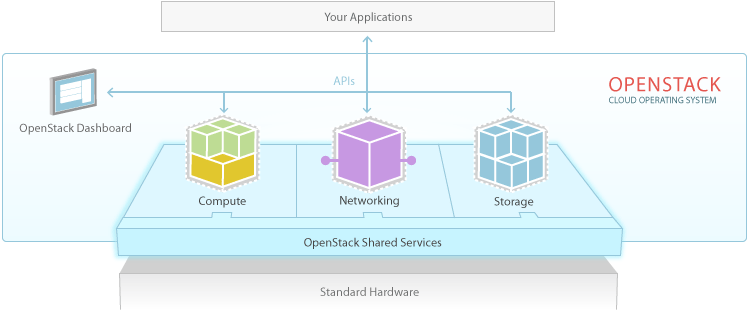
\includegraphics[width=1.0\linewidth]{openstack}
  \caption{OpenStack software diagram}\label{fig:openstack}
\end{figure}

The technology behind OpenStack consists of a series of interrelated projects delivering various components for a cloud infrastructure solution. Each service provides an open API so that all of these resources can be managed through a dashboard that gives administrators control while empowering users to provision resources through a web interface, a command-line client, or software development kits that support the API.

OpenStack is designed for horizontal scalability, so the user can easily add new compute, network, and storage resources to grow their cloud over time. In addition to the pervasiveness of massive OpenStack public clouds, many organizations, such as PayPal, Intel, and Comcast, build large-scale private clouds. OpenStack offers much more than a typical software package because it lets the user to integrate a number of different technologies to construct a cloud. This approach provides great flexibility, but the number of options might be daunting at first.

OpenStack clouds are powered by various OpenStack projects.
The selection of the components in openstack depends on how will the user be using OpenStack:

\begin{figure}[H]
  \centering
  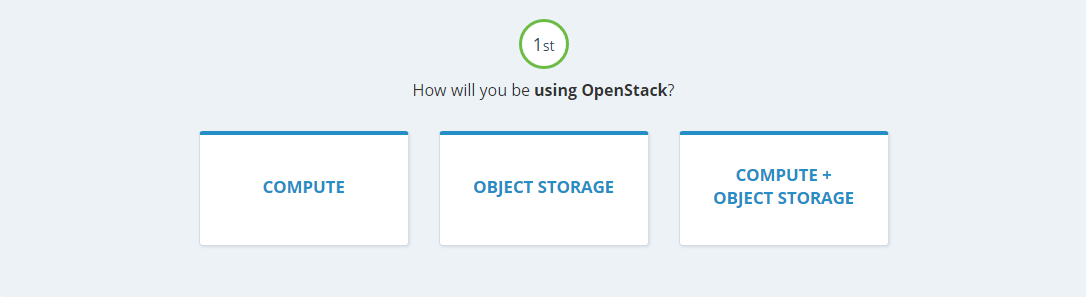
\includegraphics[width=1.0\linewidth]{Compute_ObjectStorage}
  \caption{Primary objective to decide the purpose of having an OpenStack Cloud}\label{fig:Compute_ObjectStorage}
\end{figure}

It actually specifies if the usage of OpenStack is, only with Compute - which defines the management of virtual machines on cloud, or only with Object Storage - which defines the allocation of end user based storage space on cloud, or the mix of both of Compute and Object Storage. Based on the objective of setting up the cloud, the core components can be selected as per the need from the wide range of available components.

\section{Motivation}\label{sec:motivation}

%\hint{Keep Scrolling!}\blindtext[1]
\comment{%
  \begin{itemize}
    \item The primary motivation the document is filled with huge amounts of blindtext, showing all the fancy stuff of \LaTeX{} and this template
    \item Go on scrolling though the document to find all the bells and wistles
    \item remove it, fill with your knowledge
    \item adapt the structure to your needs
  \end{itemize}
}
\blindlist{itemize}[3]
\blindtext[1]

\section{Ziel der Arbeit}\label{sec:ziel}

\blindtext[1]

\begin{figure}[htpb]
  \centering
  
\includegraphics[width=0.3\linewidth]{BildTBD}
  \caption{Hier könnte ein Bild stehen}\label{fig:bildtbd}
\end{figure}

Auch zeigt \cref{fig:bildtbd}, dass es genau so ist. Man könnte das auch mit einer \gls{gls:app}
realisieren. \missing{Quelle des Bildes noch ergänzen.}

\section{Struktur der Arbeit}\label{sec:struktur}

Die Arbeit gliedert sich wie folgt. \Cref{ch:grundlagen} erläutert wesentliche Grundlagen. Die theoretischen
Überlegungen zur Arbeit werden in \cref{ch:theorie} dargestellt. Die vorgenommene Entwicklung ist in \cref{ch:impl}
wiedergegeben.  \Cref{ch:Conclusion} fasst die Ergebnisse der Arbeit noch einmal zusammen und gibt einen Ausblick auf
zukünftige Entwicklungen.


% vim: ts=2:sw=2:sts=2:expandtab:wrapmargin=2:tw=120


% !TEX root       = ./type_name.tex
% !TEX program    = pdflatex
% !TEX encoding   = utf-8
% !TeX spellcheck = en_GB
%=======================================================================

\chapter{Introduction to Cloud Computing}\label{ch:introduction_cloud}
\sffamily{}
"Moving to the cloud", "running in the cloud", "stored in the cloud", "accessed from the cloud", these days it is probably seen that most of the activities are happening in "the cloud". If any person would like to share their data, for example digital documents, software source code, software, pictures or any videos, it is normally said to share them over "the cloud". But what exactly is this "The Cloud" and why is this "The Cloud" so important?

The short answer is that, "the cloud" is somewhere at the other end of the user's Internet connection, a place where any user can access applications and services, and where user's data can be stored securely by using any device connected over the Internet. "The cloud" is the delivery of the on-demand request of computing resources, everything and anything from applications, tools, storage, to data centres, over the Internet on a pay-for-use basis.

The Cloud is important because, there appears to be a shift going on from office-based work to working on the move. Where in the past, people would run applications or programs from software downloaded on a physical computer or server in their building, cloud computing allows people to access the same kinds of applications over the internet. The convenience of the hand held devices enabled with high speed Internet, enables the people to bridge the gap of accessing either data stored remotely or run any system or machine remotely with ease.

\comment{
The cloud is a big deal for given reasons:
\begin{itemize}
	\item It does not need any effort on the consumer or the end user's part to maintain or manage it.
	\item Any authenticated user can access the cloud-based applications and services from anywhere. All that the user needs is a device with an Internet connection.
	\item It is effectively infinite in size, so that the consumer or the end user doesn't need to worry about it running out of capacity.
	\item The resources can be scaled up or down quickly and easily to meet the desired changing demands of the consumer.
	\item The services offered in the cloud are metered services, so the end user pay only for what they use.
\end{itemize}
}

\section{Where did the cloud come from?\cite{salesforce} }\label{sec:history}

The Internet has its roots in the 1960's. But not until the early 1990's that it had any relevance for businesses. The World Wide Web (WWW) was born in 1991, and in 1993 a web browser called Mosaic was released that allowed users to view web pages that included graphics as well as text. This heralded the first company web sites – and not surprisingly, most of these belonged to companies involved in computing and technology.

As Internet connections got faster and more reliable, a new type of company called an "Application Service Provision" or ASP started to appear. ASPs took the existing business applications and ran them for their customers. The ASP would buy the computing hardware and keeping the application running, and the customer would pay a monthly fee to access it over the Internet.

But it wasn't until right at the end of the 1990's that cloud computing as it is known today did appear. That is when a company by name "salesforce.com" in 1999 introduced its own multi-tenant application which was specifically designed:
\begin{itemize}
	\item to run "in the cloud";
	\item to be accessed over the Internet from a web browser;
	\item to be used by large numbers of customers simultaneously at low cost.
\end{itemize}
Since then the cloud has enormously grown and is still growing.

\section{Services of "The Cloud"\cite{IBMcloud}}\label{sec:service_models}
The Cloud is a very broad concept, and it covers just about every possible sort of online service. Anything as a service normally abbreviated as XaaS, provided remotely can be generalised as a cloud service. But when businesses refer to \textbf{"cloud procurement"}, there are usually three models of cloud services under consideration:
\begin{itemize}
	\item \textbf{Software as a Service (SaaS)}
	\item \textbf{Platform as a Service (PaaS)}
	\item \textbf{and Infrastructure as a Service (IaaS)}
\end{itemize}

The cloud infrastructure as a service model can also be segregated based on the type of cloud network desired by the business which can be:
\begin{itemize}
	\item Private cloud: with a cloud network accessible by limited and restricted permission to only particular organisation.
	\item Public cloud: with a cloud network accessible to the general public.
	\item and Hybrid cloud: which is partly private and secured, and partly public and accessible.
\end{itemize}

\begin{figure}[H]
	\begin{center}
		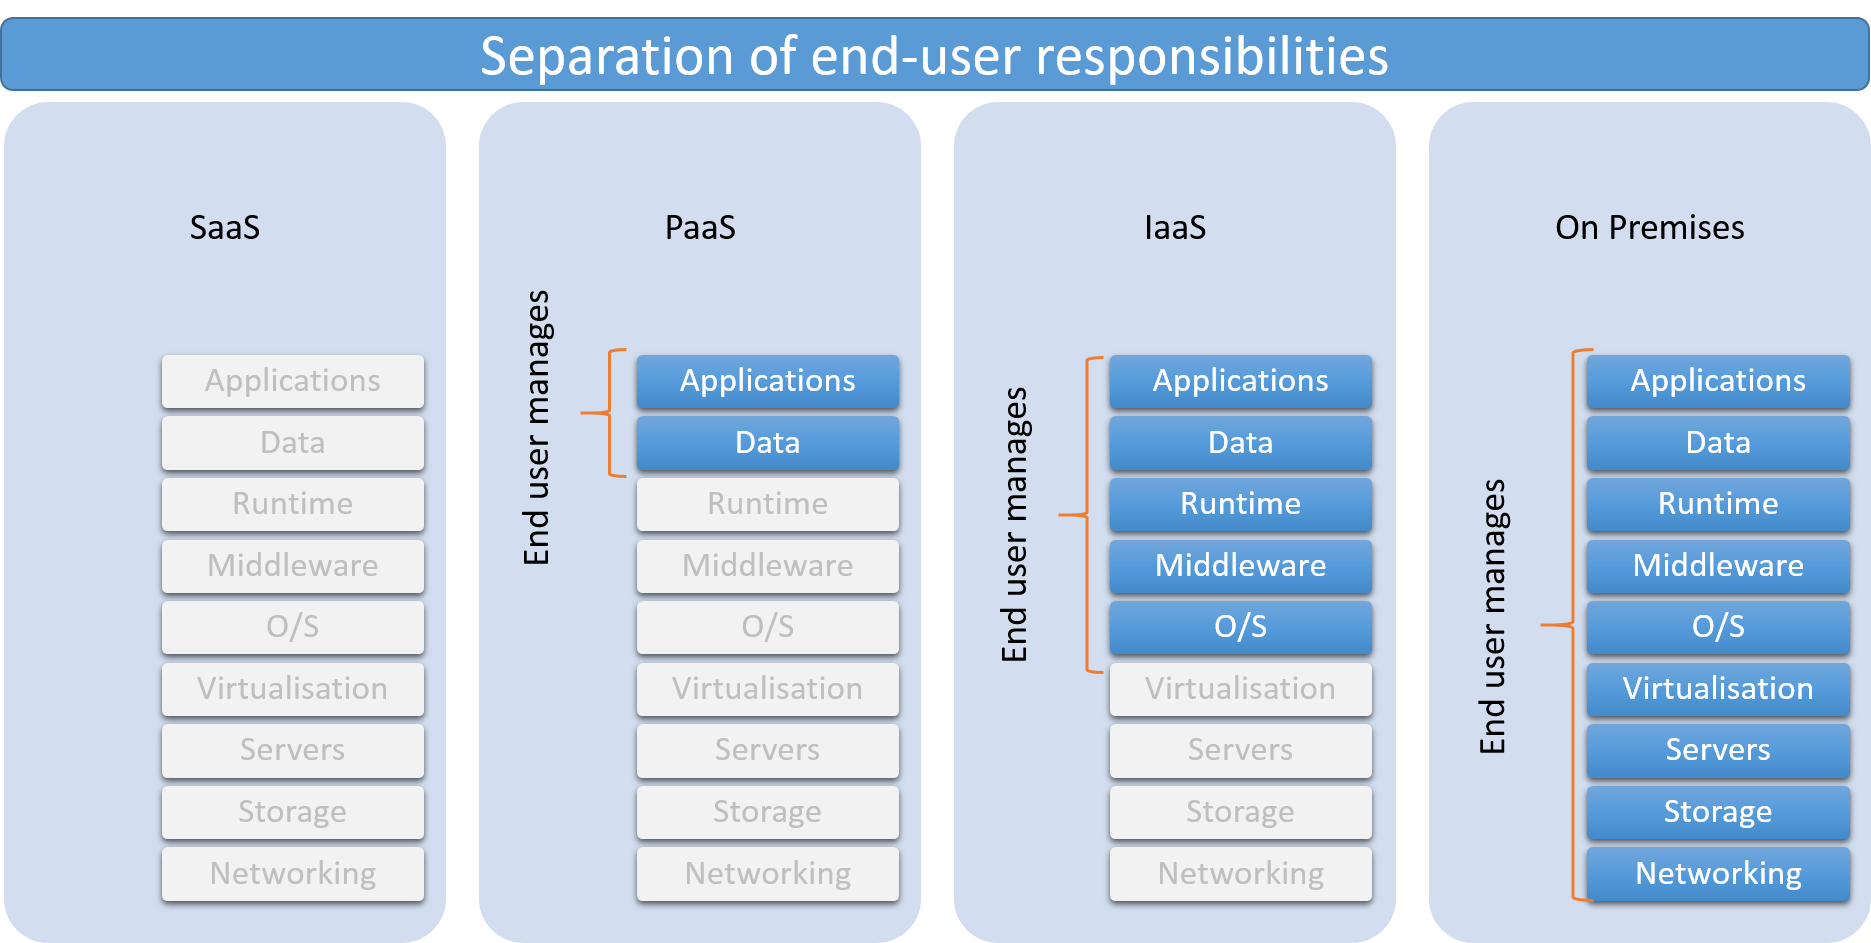
\includegraphics[width=1\linewidth]{responsibilities}
		\caption{Separation of end user responsibilities based on Internet cloud service model}
		\label{fig:responsibilities}
	\end{center}
	\vspace{-10pt}
\end{figure}

The figure \ref{fig:responsibilities} about the cloud service model describes what would be the roles that needs to be played by an end user to utilise and manage each type of service model compared to working on on-premise systems.

\subsection{Software as a Service (SaaS)}\label{ssec:SaaS}
Software as a service (SaaS) is a software distribution model in which a third-party provider hosts the applications and makes them available to customers over the Internet. Cloud-based applications or software as a service, run on distant computers "in the cloud" that are owned and operated by others and that connect to the user's computer via the Internet and, usually, a web browser.

\begin{figure}[H]
	\begin{center}
		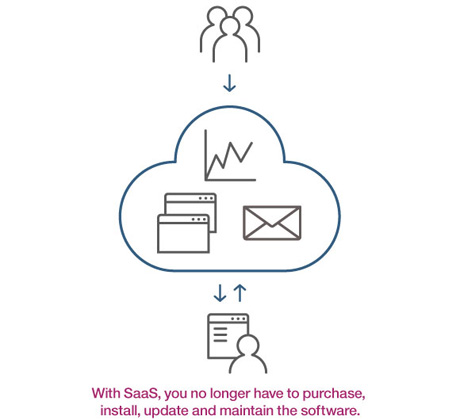
\includegraphics[width=0.95\linewidth]{cc_SaaS}
		\caption{Software as a service model\cite{IBMcloud:SaaS}}
		\label{fig:cc_SaaS}
	\end{center}
	\vspace{-10pt}
\end{figure}

SaaS is the most familiar form of cloud service for consumers. SaaS moves the task of managing software and its deployment to third-party services. Among the most familiar SaaS applications for business are customer relationship management applications like Salesforce, productivity software suites like Google Apps, and storage solutions like Box and Dropbox.

Use of SaaS applications tends to reduce the cost of software ownership by removing the need for technical staff to manage the installation, maintenance, and upgrade software, as well as reduce the cost of licensing software. SaaS applications are usually provided on a subscription model.

To summarise the benefits of SaaS:
\begin{itemize}
	\item The end user can sign up and rapidly start using innovative business apps
	\item Apps and data are accessible from any device connected to Internet
	\item No data is lost if the user's computer or a device breaks, as the data is in the cloud
	\item The service is able to dynamically scale to the usage needs
\end{itemize}

\subsection{Platform as a Service (PaaS)}\label{ssec:PaaS}
Platform as a service (PaaS) is a cloud computing model that delivers development and management tools or applications over the Internet. In a PaaS model, a cloud provider delivers hardware and software tools, "usually those needed for application development", to its users as a service. The provider of the PaaS hosts the hardware and software on their own infrastructure. As a result, PaaS frees the users from having to install in-house hardware and software to develop and run a new application.

It provides a cloud-based environment with everything required to support the complete lifecycle of building and delivering web-based (cloud) applications, without the cost and complexity of buying and managing the underlying hardware, software, provisioning, and hosting. The PaaS provider on request can provide a web development tool or platform which can be customised for the end user.


\begin{figure}[H]
	\begin{center}
		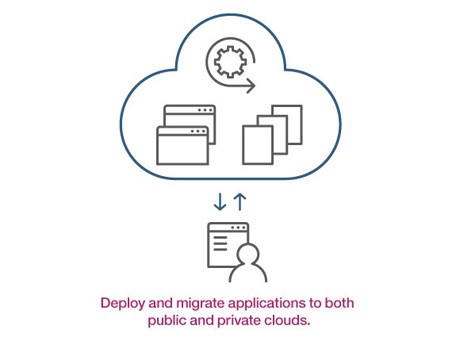
\includegraphics[width=0.95\linewidth]{cc_PaaS}
		\caption{Platform as a service model\cite{IBMcloud:PaaS}}
		\label{fig:cc_PaaS}
	\end{center}
	\vspace{-10pt}
\end{figure}

For example, deploying a typical business tool locally might require an IT team to buy and install hardware, operating systems, middleware (such as databases, Web servers and so on) the actual application, define user access or security, and then add the application to existing systems management or application performance monitoring (APM) tools. IT teams must then maintain all of these resources over time. A PaaS provider, however, supports all the underlying computing and software; users only need to log in and start using the platform – usually through a Web browser interface.

Common PaaS vendors include Salesforce.com's Force.com, which provides an enterprise customer relationship management (CRM) platform. PaaS platforms for software development and management include Appear IQ, Mendix, Amazon Web Services (AWS) Elastic Beanstalk, Google App Engine and Heroku.

To summarise the benefits of PaaS:
\begin{itemize}
	\item Develop applications and get to market faster
	\item Deploy new web applications to the cloud in minutes
	\item Reduce complexity with middleware as a service
\end{itemize}

\subsection{Infrastructure as a Service (IaaS)}\label{ssec:IaaS}

Infrastructure as a Service (IaaS) is a form of cloud computing that provides virtualized computing resources over the Internet. Infrastructure as a service provides consumers with computing resources including servers, networking, storage, and data center space on a pay-per-use basis.

\begin{figure}[H]
	\begin{center}
		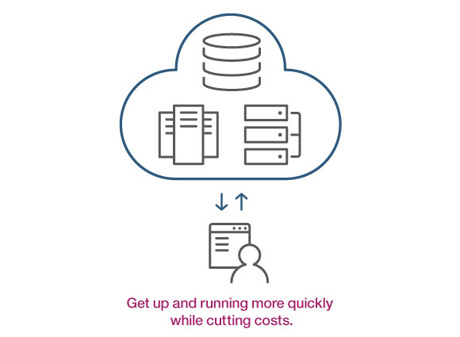
\includegraphics[width=0.95\linewidth]{cc_IaaS}
		\caption{Infrastructure as a service model\cite{IBMcloud:IaaS}}
		\label{fig:cc_IaaS}
	\end{center}
	\vspace{-10pt}
\end{figure}

In an IaaS model, a third-party provider hosts hardware, software, servers, storage and other infrastructure components on behalf of its users. IaaS providers also host users' applications and handle tasks including system maintenance, backup and resiliency planning.

IaaS platforms offer highly scalable resources that can be adjusted on-demand. This makes IaaS well-suited for workloads that are temporary, experimental or change unexpectedly.

Other characteristics of IaaS environments include the automation of administrative tasks, dynamic scaling, desktop virtualization and policy-based services.

For example, if a business is developing a new software product, it might be more cost-effective to host and test the application through an IaaS provider. Once the new software is tested and refined, it can be removed from the IaaS environment for a more traditional in-house deployment or to save money or free the resources for other projects.

Leading IaaS providers include Amazon Web Services (AWS), Windows Azure, Google Compute Engine, Rackspace Open Cloud, IBM SmartCloud Enterprise and ProfitBricks.
To summarise the benefits of IaaS:
\begin{itemize}
	\item No need to invest in having or owning the hardware
	\item Infrastructure scales on demand to support dynamic workloads
	\item Flexible, innovative services available on demand
\end{itemize}

\section{Summary about "The Cloud"}\label{sec:intro1_summary}
The cloud has become a key enabler for today's small or medium sized business to unlock creativity, drive unrivaled innovation and level the competition with larger enterprise competitors.

Prior to the advent of cloud-based products software solutions delivered over the Internet companies were often forced to invest in servers and other products to run software and store data. The advent of cloud services as well as their steady improvement in such areas as security and reliability make these solutions a logical choice for business owners and principals who want the latest innovations, functionality, and efficiency as well as cost effectiveness.

Many businesses garner considerable cost savings by migrating their software systems to the cloud. In addition to reducing reliance on the purchase and maintenance of servers, companies often lower their information technology costs in such areas as dedicated personnel and software upgrades. Most cloud services upgrade and update software via the Internet with little or no downtime for end users, decreasing the wait time associated with installing and testing software on an on-site network. Moreover, cloud-based products are scalable: unlike conventional software, cloud services can be expanded as needed to encompass as many end users as required without additional overhead of servers and upgrades to handle added workloads.

When more number of small and medium sized business begin to realize that the cloud can do more than just reduce the cost of IT, the journey to the cloud becomes inevitable and the question shifts from whether to adopt cloud technologies to how to do so sensibly.

It is fascinating to understand the working of cloud as it has created lot of new opportunities for research, jobs and investment in this domain.
% !TEX root       = ./type_name.tex
% !TEX program    = pdflatex
% !TEX encoding   = utf-8
% !TEX spellcheck = de_DE_frami
%=======================================================================

%\chapter{Introduction}\label{ch:einleitung}
\chapter{Introduction to OpenStack Cloud\cite{OpenStack}}\label{ch:introduction_openstack}
\sffamily{}
An introduction about cloud computing and its different offering of service modelling was introduced in the chapter \nameref{ch:introduction_cloud}. This chapter \nameref{ch:introduction_openstack} introduces about one of the open source IaaS cloud operating system called OpenStack.

OpenStack is a cloud operating system that controls large pools of compute, storage, and networking resources throughout a datacenter, all managed through a dashboard that gives administrators control while empowering their users to provision resources through a web interface.

OpenStack is the open source cloud computing platform that meets the needs of public and private cloud providers regardless of size. OpenStack services control large pools of compute, storage, and networking resources throughout a data center. The figure \ref{fig:openstack} shows the basic overview of core services in OpenStack.

\begin{figure}[H]
  \centering
  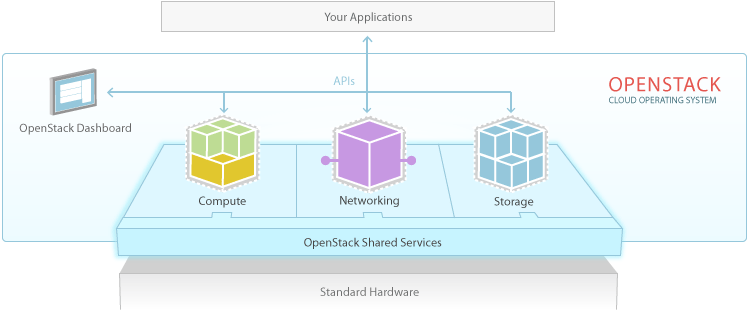
\includegraphics[width=1.0\linewidth]{openstack}
  \caption{OpenStack software diagram\cite{OpenStack:software}}
  \label{fig:openstack}
\end{figure}

The technology behind OpenStack consists of a series of interrelated projects delivering various components for a cloud infrastructure solution. Each service provides an open API so that all of these resources can be managed through a dashboard that gives administrators control while empowering users to provision resources through a web interface, a command-line client, or software development kits that support the API.

OpenStack is designed for horizontal scalability, so the user can easily add new compute, network, and storage resources to grow their cloud over time. In addition to the pervasiveness of massive OpenStack public clouds, many organizations, such as PayPal, Intel, and Comcast, build large-scale private clouds. OpenStack offers much more than a typical software package because it lets the user to integrate a number of different technologies to construct a cloud. This approach provides great flexibility, but the number of options might be daunting at first.

OpenStack clouds are powered by various OpenStack projects.
The selection of the components in openstack depends on how does the IaaS provider wants to use the OpenStack:

\begin{figure}[H]
  \centering
  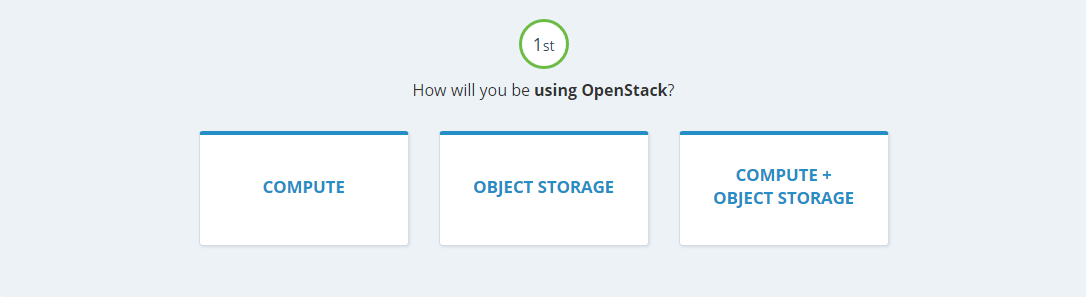
\includegraphics[width=1.0\linewidth]{Compute_ObjectStorage}
  \caption{Primary objective to decide the purpose of having an OpenStack Cloud\cite{OpenStack}}\label{fig:Compute_ObjectStorage}
\end{figure}

The figure \ref{fig:Compute_ObjectStorage} actually specifies if the primary objective of the usage of OpenStack is, only with Compute - which defines the management of virtual machines on cloud, or only with Object Storage - which defines the allocation of end user based storage space on cloud, or the mix of both of Compute and Object Storage. Based on the objective of setting up the cloud, the core components can be selected as per the need from the wide range of available components.

\section{Architecture of OpenStack}\label{sec:architecture}
The OpenStack project is an open source cloud computing platform that aims for simple implementation, massive scalability, and a rich set of features. Cloud computing experts from around the world contribute to the project.

OpenStack provides an Infrastructure-as-a-Service (IaaS) solution through a variety of complemental services. Each service offers an application programming interface (API) that facilitates this integration.

\begin{figure}[H]
	\begin{center}
		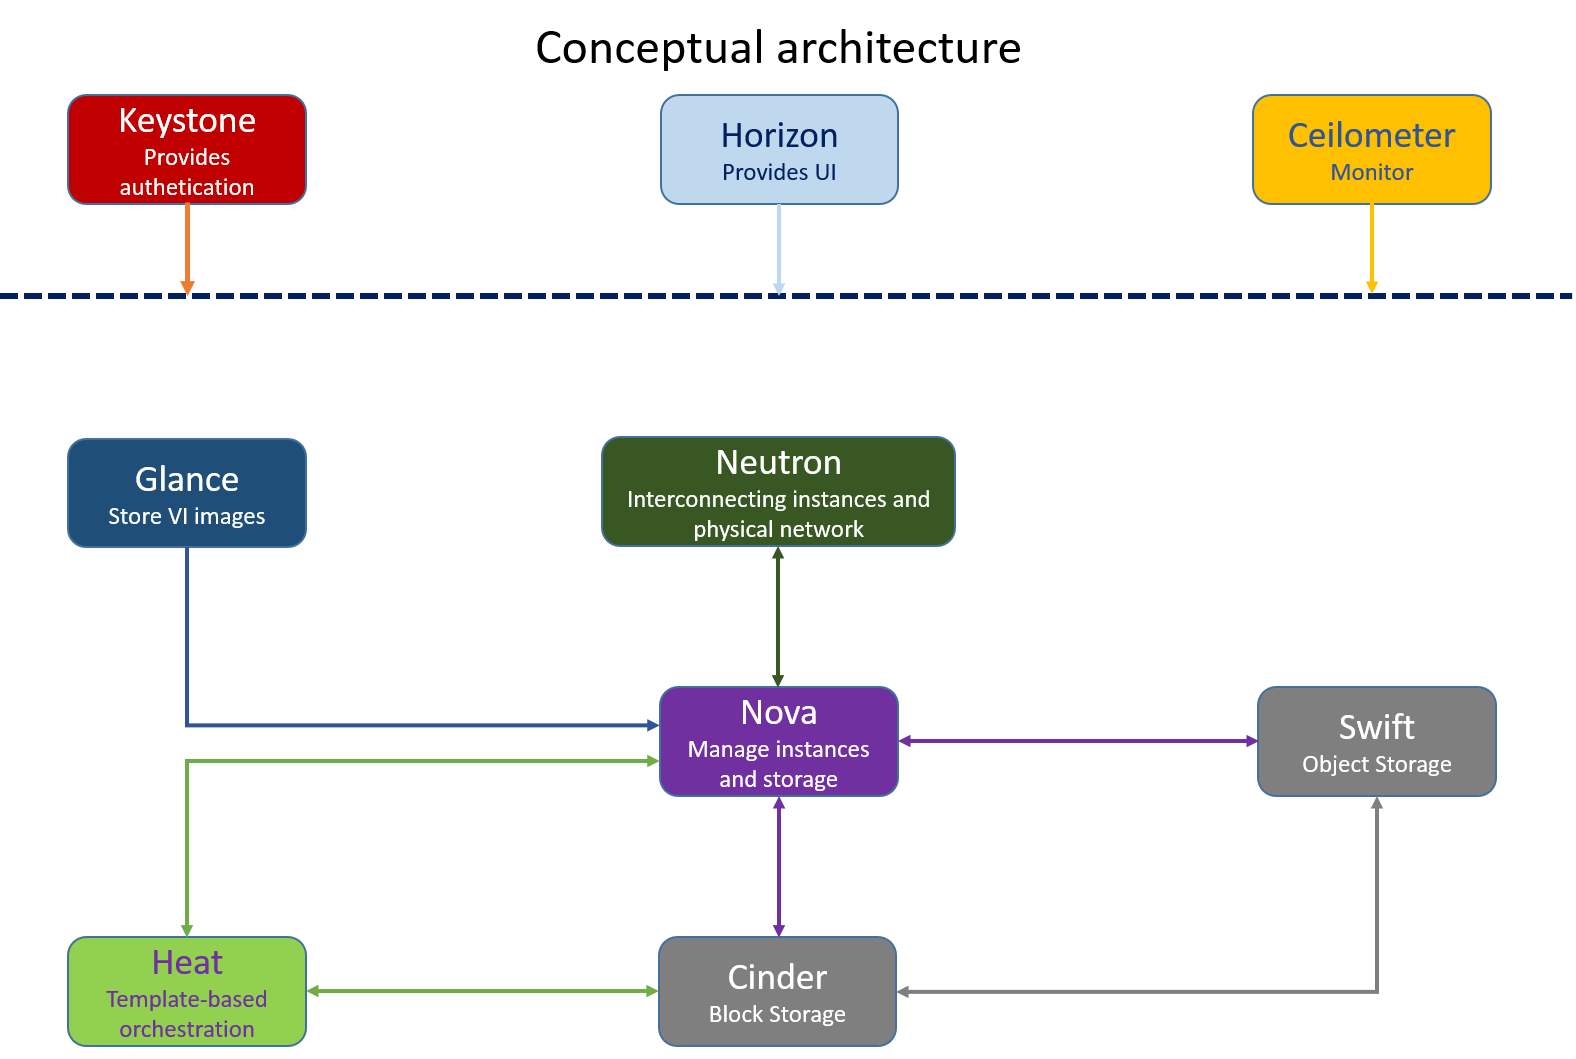
\includegraphics[width=1.0\linewidth]{conceptual_architecture}
		\caption{The relationships among the OpenStack services}\label{fig:openstack_architecture}
	\end{center}
	\vspace{-10pt}
\end{figure}

The figure \ref{fig:openstack_architecture} shows the architecture of the services and how each service communicates with the other services and provide the desired cloud solution.

The implementation of the services are based on the objective of having the OpenStack cloud.
Each purpose of cloud solution have their own set of service requirements that needs to be installed on the nodes and enabled.

\subsection{OpenStack for compute}\label{ssec:openstackforcompute}
To set up the OpenStack for the purpose of Compute, it would require the implementation of the following services:
\begin{itemize}
  \item Identity service (Keystone) -- core service
  \item Compute service (Nova) -- core service
  \item Networking service (Neutron) -- core service
  \item Block storage service (Cinder) -- core service
  \item Image service (Glance) -- core service
  \item Dashboard service (Horizon) -- optional
  \item Telemetry service (Ceilometer) -- optional
\end{itemize}

\subsection{OpenStack for storage}\label{ssec:openstackforstorage}
To set up the OpenStack for the purpose of storage, it would require the implementation of the following services:
\begin{itemize}
  \item Object storage service (Swift) -- core service
  \item Identity service (Keystone) -- core service
  \item Dashboard service (Horizon) -- optional
  \item Telemetry service (Ceilometer) -- optional
\end{itemize}


\subsection{Description of the core services in OpenStack}\label{ssec:openstackservices}
\begin{itemize}
  \item Compute service (Nova) - Manages the lifecycle of compute instances in an OpenStack environment. Responsibilities include spawning, scheduling and decomissioning of machines on demand.
  \item Object storage service (Swift) - Stores and retrieves arbitrary unstructured data objects via a RESTful, HTTP based API. It is highly fault tolerant with its data replication and scale out architecture. Its implementation is not like a file server with mountable directories.
  \item Networking service (Neutron) - Enables network connectivity as a service for other OpenStack services, such as OpenStack Compute. Provides an API for users to define networks and the attachments into them. Has a pluggable architecture that supports many popular networking vendors and technologies.
  \item Image service (Glance) - Stores and retrieves virtual machine disk images. OpenStack Compute makes use of this during instance provisioning.
  \item Identity service (Keystone) - Provides an authentication and authorization service for other OpenStack services. Provides a catalog of endpoints for all OpenStack services.
  \item Dashboard service (Horizon) - Provides a web-based self-service portal to interact with underlying OpenStack services, such as launching an instance, assigning IP addresses and configuring access controls.
  
  
  \item Telemetry service (Ceilometer) - Monitors and meters the OpenStack cloud for billing, benchmarking, scalability, and statistical purposes.
  \item Block storage service (Cinder) - Provides persistent block storage to running instances. Its pluggable driver architecture facilitates the creation and management of block storage devices.
  \item Orchestration service (Heat) - Orchestrates multiple composite cloud applications by using either the native HOT template format or the AWS CloudFormation template format, through both an OpenStack-native REST API and a CloudFormation-compatible Query API.
\end{itemize}

The thesis is more focussed on the understanding of the nova compute service and the nova filter scheduler, and this would be documented further in the next sections the \nameref{sec:novacompute} and the \nameref{sec:novafilterschedulerdetailed}.

\section{OpenStack Nova Compute}\label{sec:novacompute}
Nova is an OpenStack project designed to provide power massively scalable, on demand, self service access to compute resources.
Nova enables the lifecycle management of the virtual machines by provisioning or managing the resources for creation, management or deletion of virtual machines.

Nova is further segregated into many sub modules based on the defined purpose like segregation of nodes, scheduling mechanism, management of virtual machines.

\subsection{Host Aggregates}\label{ssec:hostaggregates}
Nova enables the segregation of nova nodes by categorizing them into "Availability Zones" by the use of Host Aggregates mechanism.
This mechanism helps to further divide resources based on Availability Zones. Host aggregates are visible only to the administrators whereas Availability zones are visible to the users. This information is used by the nova scheduler as to enable advanced scheduling or to define any logical groups for creation or migration of virtual machines.

\subsection{Threading model}\label{ssec:threadingmodel}
All OpenStack services use the green thread model of threading which reduces the likelihood of race conditions. In case of any code taking longer execution time and blocking any other threads for execution, an added eventlet code from the greenthread library will hlp to switch to process any pending threads.

\subsection{Virtual Machine States and Transitions}\label{ssec:VirtualMachineStatesTransitions}
Nova manages the state transitions of virtual machine throughtout the lifecycle from creation to deletion or handle any error states.
When the creation of an instance is requested, the nova allocates the compute node for hosting the instance and enters the initial state of "building" and spawns the virtual instance unless there are any errors which would lead to the transition of the state to "error". As shown in \textit{Figure} \ref{fig:statetransitionsdiagram}, it provides the information about different transitional states along with the possible change of state instance state.

\begin{figure}[H]
	\begin{center}
		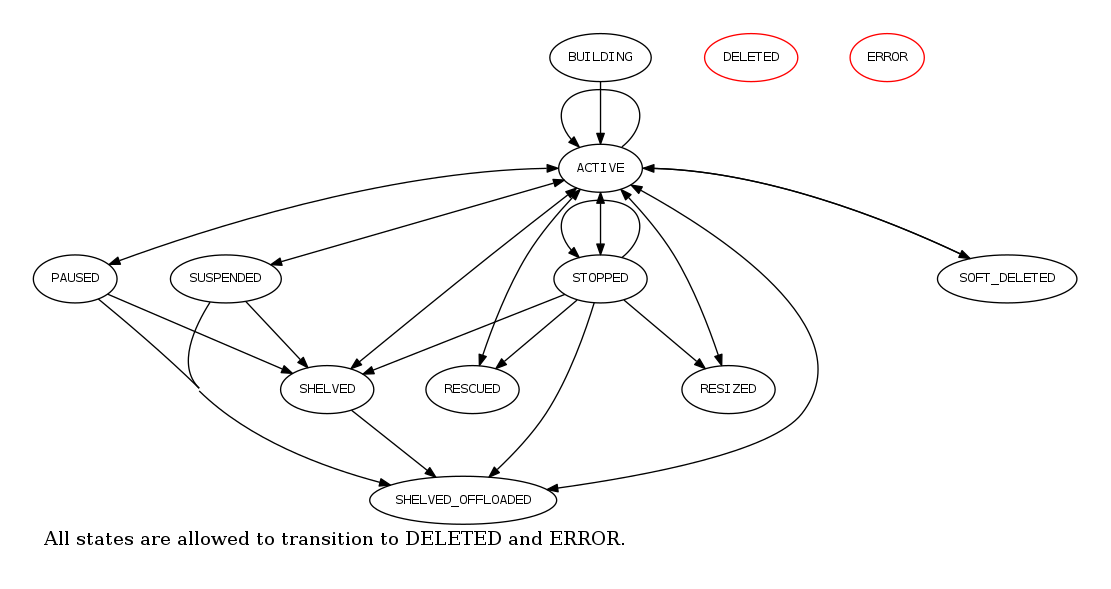
\includegraphics[width=1.0\linewidth]{state_transitions_diagram}
		\caption{The diagram shows the allowed different state transistions of a virtual machine\cite{OpenStack:state_transitions}}\label{fig:statetransitionsdiagram}
	\end{center}
	\vspace{-10pt}
\end{figure}

\subsection{Filter Scheduler}\label{ssec:filterschedulermin}
Nova has its own scheduling mechanism called "Filter Scheduler" which computes the placement decision of creation or migration of virtual instances.
The scheduler is further explained in detail in the section \nameref{sec:novafilterschedulerdetailed}.

\subsection{Advanced Message Queue Protocol and Nova}\label{ssec:amqpnova}
The Advanced Message Queue Protocol (AMQP) is the messaging technology chosen by OpenStack to communicate between different nodes using a message queue enabler like RabbitMQ or Qpid.
The nova components use the Remote Procedure Calls(RPC hereinafter) to communicate to one another. The RPC calls are authenticated for communication using message queue enabler like rabbitMQ, which validates the authentication using Keystone.

\subsection{Block Device Mapping}\label{ssec:blockdevicemapping}
Nova has a concept of block devices that can be exposed to cloud instances.
Block device mapping is a way to organize and keep data about all of the block devices an instance has.

\subsection{Nova OpenStack RESTful API}\label{ssec:novarestapi}
The Nova provides the RESTful API which is exposed as an HTTP request service for routing, controllers and actions, serialization and trigering faults.

\subsection{Conductor}\label{ssec:novaconductor}
Conductor serves as a database proxy, object backporter and also as a centralized place to manage the execution of workflows which involve the scheduler.

\subsection{Notifications in Nova}\label{ssec:novanotifications}
Similarly to other OpenStack services Nova emits notifications to the message bus with the Notifier class provided by oslo.messaging.

\section{Standard Nova Filter Scheduler}\label{sec:novafilterschedulerdetailed}
The \textbf{Filter Scheduler} supports filtering and weighting to make informed decisions on where a new instance should be created.
This Scheduler supports working with Compute Nodes only.
\begin{figure}[H]
	\begin{center}
		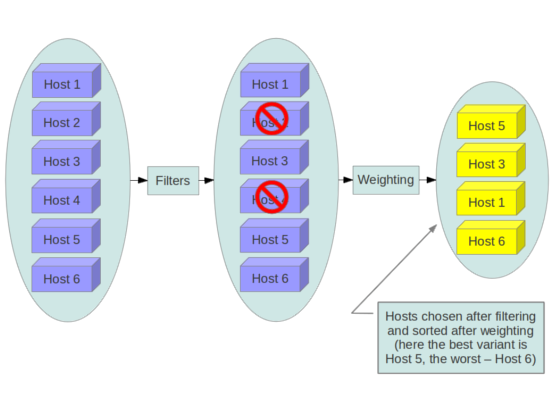
\includegraphics[width=1\linewidth]{filteringWorkflow1}
		\caption{Filtering the compute hosts and sorting them based on weights\cite{OpenStack:filteringworkflow1}}\label{fig:filteringWorkflow1}
	\end{center}
	\vspace{-10pt}
\end{figure}
The filter scheduler iterates over all the available compute nodes, evaluates each compute node against the set of filters, and a list of the possible nodes for instance creation is generated sorted based on the weights.
The scheduler then chooses the best host for the instance by choosing the most weighted host. For any specific filter to pass a specific host, the filter matches the users request against the state of the host as defined by each filter definition.

If the scheduler does not find any hosts and returns an empty set of list of hosts for any requested instance, it means that there is no possible host where the instance can be placed to complete the user request.

The filter scheduler has to be flexible to support the required variety of filtering and weighting strategies. The nova also permits to implement the user's own filtering algorithm.

\subsection{Filtering}\label{ssec:novafiltering}
There are many standard filter classes which may be used (nova.scheduler.filters):
\begin{itemize}
    \item \textbf{AllHostsFilter} - The initial hosts filter to pass all the available hosts.

    \item \textbf{ImagePropertiesFilter} - This filters the possible hosts based on properties defined by the instance's image. It passes hosts that can support the properties specified on the image used by the instance.

    \item \textbf{AvailabilityZoneFilter} - This filters the hosts which are grouped by availability zone. It passes only those hosts which match the availability zone specified in the instance properties.

    \item \textbf{ComputeCapabilitiesFilter} - This filter checks that if the capabilities provided by the host compute service satisfy any extra specifications associated with the instance type. It passes hosts that can create the specified instance type.

    \item \textbf{ComputeFilter} - This passes all the hosts that are operational and enabled.

    \item \textbf{CoreFilter} - This filters the hosts based on available VCPU cores. It passes hosts with sufficient number of CPU cores.

    \item \textbf{AggregateCoreFilter} - This filters the hosts by CPU core number with \\per-aggregate \verb|cpu_allocation_ratio| setting specified in the nova configuration. If no per-aggregate value is found, it will fall back to the global default \verb|cpu_allocation_ratio|.

    \item \textbf{IsolatedHostsFilter} - This filter is based on \verb|image_isolated|, \verb|host_isolated| and \verb|restrict_isolated_hosts_to_isolated_images| flags.

    \item \textbf{JsonFilter} - This filter allows simple JSON-based grammar for selecting hosts.

    \item \textbf{RamFilter} - This filters the hosts by their available RAM capacity. Only those hosts with sufficient RAM capacity to host the instance are passed.

    \item \textbf{AggregateRamFilter} - This filters the hosts by RAM with per-aggregate \\\verb|ram_allocation_ratio| setting specified in the nova configuration. If no per-aggregate value is found, it will fall back to the global default \\\verb|ram_allocation_ratio|. 

    \item \textbf{DiskFilter} - This filters the hosts by their storage space. Only hosts with sufficient storage space to host the instance are passed.

    \item \textbf{AggregateDiskFilter} - This filters the hosts by disk allocation with per-aggregate \verb|disk_allocation_ratio| setting. If no per-aggregate value is found, it will fall back to the global default \verb|disk_allocation_ratio|.

    \item \textbf{NumInstancesFilter} - This filters the compute nodes by number of running instances. Nodes with too many instances will be filtered out.

    \item \textbf{AggregateNumInstancesFilter} - This filters the hosts by number of instances with per-aggregate \verb|max_instances_per_host| setting.

    \item \textbf{IoOpsFilter} - This filters the hosts by concurrent I/O operations on it. The hosts with too many concurrent I/O operations will be filtered out.

    \item \textbf{AggregateIoOpsFilter} - filters hosts by I/O operations with per-aggregate \verb|max_io_ops_per_host| setting. If no per-aggregate value is found, it will fall back to the global default \verb|max_io_ops_per_host|.

    \item \textbf{PciPassthroughFilter} - This filter schedules instances on a host if the host has devices to meet the device requests in the \verb|‘extra_specs’| for the flavor.

    \item \textbf{SimpleCIDRAffinityFilter} - This filter allows a new instance on a host within the same IP block.

    \item \textbf{DifferentHostFilter} - This filter allows the instance on a different host from a set of instances.

    \item \textbf{SameHostFilter} - This filter puts the instance on the same host as another instance in a set of instances.

    \item \textbf{RetryFilter} - This filters the hosts that have been attempted for scheduling. Only passes hosts that have not been previously attempted.

    \item \textbf{TrustedFilter} (EXPERIMENTAL) - This filters the hosts based on their trust. Only passes hosts that meet the trust requirements specified in the instance properties.

    \item \textbf{TypeAffinityFilter} - Only the hosts that are not already running an instance of the requested type are passed.

    \item \textbf{AggregateTypeAffinityFilter} - This limits \verb|instance_type| by aggregate.

    \item \textbf{ServerGroupAntiAffinityFilter} - This filter implements anti-affinity for a server group.

    \item \textbf{ServerGroupAffinityFilter} - This filter works the same way as ServerGroupAntiAffinityFilter. The difference is that when you create the server group, you should specify a policy of ‘affinity’.

    \item \textbf{AggregateMultiTenancyIsolation} - This isolate the tenants in specific aggregates.

    \item \textbf{AggregateImagePropertiesIsolation} - This isolates the hosts based on image properties and aggregate metadata.

    \item \textbf{MetricsFilter} - This filters the hosts based on metrics \verb|weight_setting|. Only those hosts with the available metrics are passed.

    \item \textbf{NUMATopologyFilter} - This filters the hosts based on the NUMA topology requested by the instance, if any.
\end{itemize}

\subsection{Weights}\label{ssec:novaweights}
Filter Scheduler uses the weight based approach during its selection of a host for the requested instance.
A weigher is a way to select the best suitable host from a group of valid hosts by giving weights to all the hosts in the list.

In order to prioritize one weigher against another, all the weighers have to define a multiplier that will be applied before computing the weight for a node. All the weights are normalized beforehand so that the multiplier can be applied easily. Therefore the final weight for the object will be:
\begin{lstlisting}[frame=single]
weight = w1_multiplier * norm(w1) + w2_multiplier * norm(w2) + ...
\end{lstlisting}

The Filter Scheduler weighs hosts based on the config option \verb|scheduler_weight_|- \verb|classes|, this defaults to \verb|nova.scheduler.weights.all_weighers|, which selects the following weighers:

\begin{itemize}
	\item \textbf{RAMWeigher} - Compute weight based on available RAM on the compute node.

	\item \textbf{DiskWeigher} - Hosts are weighted and sorted by free disk space with the largest weight winning.

	\item \textbf{MetricsWeigher} - This weigher can compute the weight based on the compute node host’s various metrics.
		The to-be weighed metrics and their weighing ratio are specified in the configuration file as the followings:
\begin{lstlisting}[frame=single]
metrics_weight_setting = name1=1.0, name2=-1.0
\end{lstlisting}

	\item \textbf{IoOpsWeigher} - The weigher can compute the weight based on the compute node host’s workload. The default is to preferably choose light workload compute hosts.

	\item \textbf{ServerGroupSoftAffinityWeigher} - The weigher can compute the weight based on the number of instances that run on the same server group.
		The largest weight defines the preferred host for the new instance.

	\item \textbf{ServerGroupSoftAntiAffinityWeigher} - The weigher can compute the weight based on the number of instances that run on the same server group as a negative value.

	\item \textbf{IoOpsWeigher} - Hosts are weighted and sorted by free disk space with the largest weight winning.
\end{itemize}

Filter Scheduler makes a local list of acceptable hosts by repeated filtering and weighing.
Each time it chooses a host, it virtually consumes resources on it, so subsequent selections can adjust accordingly.
It is useful if the customer asks for a large block of instances, because weight is computed for each instance requested.

\begin{figure}[H]
	\begin{center}
		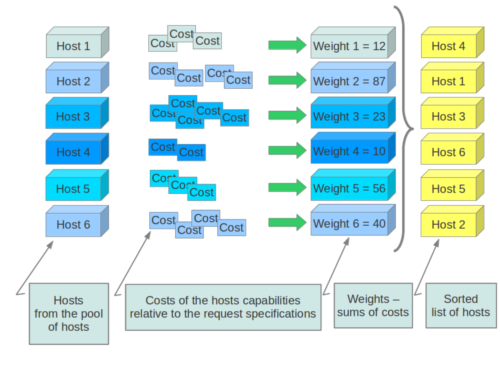
\includegraphics[width=1\linewidth]{filteringWorkflow2}
		\caption{Compute hosts sorted based on weights\cite{OpenStack:filteringWorkflow2}}\label{fig:filteringWorkflow2}
	\end{center}
	\vspace{-10pt}
\end{figure}

At the end, the Filter Scheduler sorts selected hosts by their weight and attempts to provision instances on the chosen hosts.

\section{Opening for any improvements in the filter scheduler?}\label{sec:openingforimprovement}
The filter scheduler executes the instances one instance at a time.
If an user requests for bulk creation of instances, for example: consider a request for creation of \verb|n| instances, the filter scheduler would need to run for \verb|n| number of times to execute the placement decision for each requested instance.

If the user's request for the creation of large number of instances could be modelled into a Linear programming model with the parameters that are required to filter the hosts and then computing them into a Linear programming solver like cPlex, the resultant solution could achieve better results with lesser execution time for the creation of large number of instances.

There could be many possibilities of modelling the linear programming model to have a placement decision of the host like the Virtual Network Embedding problem.
Such problems are also known as knapsack problem in combinatorial optimisation.

Given the current availability of input data, there is also no possibility of network aware scheduling which would consider the amount of network load on the host machines before placing the instance.

With the learning curve of OpenStack, there could be many possibilities to optimise and solve the instance scheduling problem based on the purpose of the cloud provider and the availability of the inputs to model the Linear program with a better scheduling approach.

\section{Structure of the thesis}\label{sec:thesisstructure}
The first chapter \nameref{ch:introduction_cloud} provides the basic concept of cloud and its offerings. This chapter \nameref{ch:introduction_openstack} gives an idea about OpenStack as an IaaS model and the brief understanding about the services offered by OpenStack.

The next chapter \nameref{ch:installationofopenstack} will explain the implementation of the services to set up the OpenStack for the purpose of computing.
The chapter \nameref{ch:novaalgorithm} would explain about the Nova Filter Scheduler and the flow of code as how the filter scheduler algorithm is invoked during creation of instances.
Then the chapter \nameref{ch:implementationofcplex} would explain the new mathematical formulation used to schedule the instances and its implementation.
In the chapter \nameref{ch:comparisionofbothscheduler} one could see and evaluate the performance between the existing filter scheduler and the new modelled scheduler algorithm followed by the chapters \nameref{ch:futurepossibilities} and \nameref{ch:Conclusion}.


%Auch zeigt \ref{fig:bildtbd}, dass es genau so ist. Man könnte das auch mit einer \gls{gls:app}
%realisieren. \missing{Quelle des Bildes noch ergänzen.}
% !TEX root       = ./type_name.tex
% !TEX program    = pdflatex
% !TEX encoding   = utf-8
% !TEX spellcheck = de_DE_frami
%=======================================================================

\chapter{Installation and Configuration of OpenStack}\label{ch:installationofopenstack}

The OpenStack consists of several key service projects which needs to be installed seperately.
These projects work together depending on the user's cloud needs.
The projects include Compute, Identity Service, Networking, Image Service, Block Storage, Object Storage, Telemetry, Orchestration, and Database.
Any services can be installed seperately and configure them stand-alone or as connected entities.

The Liberty version of OpenStack has been installed for the cloud test setup which has been documented in this thesis.
The OpenStack installation guide can also be found at \href{http://docs.openstack.org/liberty/install-guide-ubuntu/} {OpenStack Installation Guide for Ubuntu}.

The OpenStack project is an open source cloud computing platform that supports all types of cloud environments.
The project aims for simple implementation, massive scalability, and a rich set of features.
Cloud computing experts from around the world contribute to the project.

OpenStack provides an Infrastructure-as-a-Service (IaaS) solution through a variety of complemental services.
Each service offers an application programming interface (API) that facilitates this integration.


%\blindtext[1]

\section{Minimum hardware requirements for the compute purpose of the cloud}\label{sec:hardwarerequirements}
It requires at the least two nodes(hosts) to set up the OpenStack and launch a virtual machine or instance.
Optional services such as Block Storage and Object Storage require additional nodes.

The hardware architecture explained is the minimal hardware requirements for each type of node.
The figure \ref{fig:hwreqs} gives a general idea about the required nodes and optional nodes to start with an OpenStack for compute.

\begin{figure}[H]
  \centering
  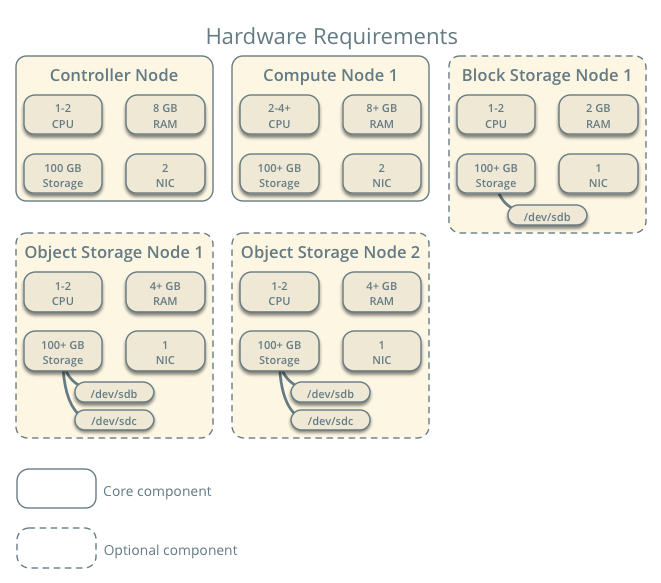
\includegraphics[width=1.0\linewidth]{hwreqs}
  \caption{Minimum hardware requirements to set up the OpenStack test bed\cite{OpenStack:hwreqs}}\label{fig:hwreqs}
  \vspace{-10pt}
\end{figure}


\subsection{Controller}\label{ssec:hwcontroller}
The \verb|controller| node runs the Identity service, Image service, management portions of Compute, management portion of Networking, various Networking agents, and the dashboard. It also includes supporting services such as an SQL database, message queue, and Network Time Protocol.

Optionally, the \verb|controller| node runs portions of Block Storage, Object Storage, Orchestration, and Telemetry services.

The \verb|controller| node requires a minimum of two network interfaces, 8 GB of RAM, 100 GB of storage space.

\subsection{Compute}\label{ssec:hwCompute}
The \verb|compute| node runs the hypervisor portion of Compute that operates instances.
By default, Compute uses the KVM hypervisor.
The \verb|compute| node also runs a Networking service agent that connects instances to virtual networks and provides firewalling services to instances via security groups.

You can deploy more than one \verb|compute| node.
Each node requires a minimum of two network interfaces,
more than 8 GB of RAM,
more than 100 GB of storage space and more than 2 CPU cores.

\subsection{Block Storage}\label{ssec:hwblockstorage}
This is an optional implementation and has not been set up for the test bed for this thesis.
The optional Block Storage node contains the disks that the Block Storage service provisions for instances.

You can deploy more than one block storage node.
Each node requires a minimum of one network interface.

\subsection{Object Storage}\label{ssec:hwobjectstorage}
This is also an optional implementation and has not been set up for the test bed for this thesis.
The optional Object Storage node contain the disks that the Object Storage service uses for storing accounts, containers, and objects.

This service requires two nodes.
Each node requires a minimum of one network interface.
You can deploy more than two object storage nodes.

\section{Networking Options}\label{sec:Networkingoptions}
OpenStack provides two diferent networking options:
\begin{itemize}
	\item Networking Option 1: Provider networks
	\\The provider networks option deploys the OpenStack Networking service in the simplest way possible with primarily layer-2 (bridging/switching) services and VLAN segmentation of networks.
	Essentially, it bridges virtual networks to physical networks and relies on physical network infrastructure for layer-3 (routing) services.
	Additionally, a DHCP service provides IP address information to instances.

	\item Networking Option 2: Self-service networks
	\\The self-service networks option augments the provider networks option with layer-3 (routing) services that enable self-service networks using overlay segmentation methods such as VXLAN.
	Essentially, it routes virtual networks to physical networks using NAT.
	Additionally, this option provides the foundation for advanced services such as LBaaS and FWaaS.
\end{itemize}

Considering the network options, the networking option 2 of self service networks have been implemented for the test bed.

%Weiterführende Informationen zu diesem Thema bietet~\cite{Herrmann2004}. In dem Buch werden auch Details zu \acp{ic}
%dargestellt.
%\blindtext[2]
%\blindenumerate{}
%\blindtext[2]

\section{Configuration of Services and config files}\label{sec:configurationofopenstack}

For the test bed of this thesis, there is one \verb|controller| node and four \verb|compute| nodes which have been configured.
All the nodes have been installed with the \verb|Ubuntu 14.04| \verb|LTS| Operating system.
For the purpose of having the GUI, the desktop version of the Operating system has been set up on each node.

This thesis does not explain the installation in detail as it is already available in \href{http://docs.openstack.org/liberty/install-guide-ubuntu/} {OpenStack Installation Guide for Ubuntu}.
This thesis covers the basics of the topics which were covered during the setup of the test bed are documented. And also, the problems that were faced due to some of the missing configurations as they were not mentioned in the \href{http://docs.openstack.org/liberty/install-guide-ubuntu/} {OpenStack Installation Guide for Ubuntu} are documented in this section.

To keep the configuration of the testbed simple, the password used for convenience on all the host machines and all the OpenStack services is \verb|user|.


\subsection{Host networking}\label{ssec:Hostnetworkingarchitecture}

\begin{figure}[H]
  \centering
  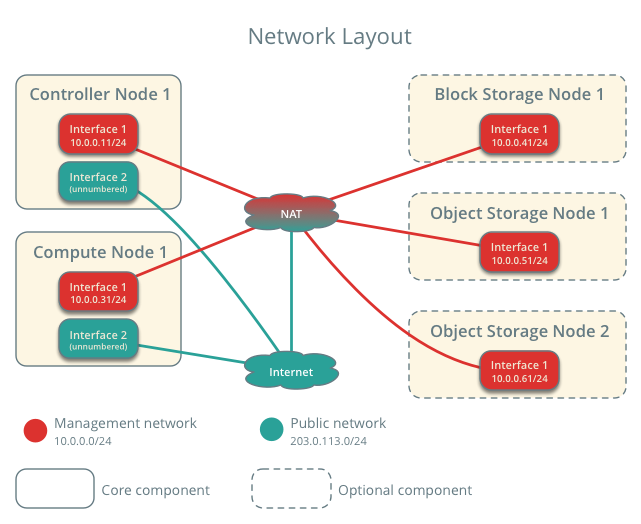
\includegraphics[width=1.0\linewidth]{networklayout}
  \caption{Network layout among all the host machines\cite{OpenStack:networklayout}}\label{fig:networklayout}
\end{figure}
The figure \ref{fig:networklayout} shows how the connections are established between all the node machines.
A private management network and a public network provided with internet connection are set up for the \verb|controller| and \verb|compute| nodes.
The management network's IP for the network interface of \verb|controller| node is set to static IP of \verb|10.0.0.11|.
Similarly, the management network's IP for one of the network interfaces on the five of the \verb|compute| nodes have the static IPs ranging from \verb|10.0.0.31| to \verb|10.0.0.35|.

In this thesis, the storage nodes have not been implemented.

For the testbed setup, one \verb|controller| node and five computes nodes have been set up.


\subsection{Network Time Protocol (NTP)}\label{ssec:NetworkTimeProtocol_NTP}
The Chrony application is installed on all the nodes to synchronise the time on all the installed nodes.
The \verb|controller| node is set to synchronise with the network time server provided by "TU-Chemnitz" given by the server host name as \verb|ntphost1.hrz.| \verb|tu-chemnitz.de|.
The other \verb|compute| nodes are set to have the synchronised time with the \verb|controller| node by setting the \verb|controller| node as network time server.

\subsection{OpenStack packages}\label{ssec:OpenStackpackages}
OpenStack packages are installed on all the nodes by enabling the OpenStack repository and installing all required basic packages.

The MariaDB SQL database server is installed on the \verb|controller| node to store the information related to OpenStack services for authentication and other related activities.
The MongoDB NoSQL database is installed on the \verb|controller| for the purpose of Telemetry service (Ceilometer).

OpenStack uses the message queue to co-ordinate operations and services among the installed services.
The RabbitMQ server is installed on the \verb|controller| node to provide the message queue service among the services.


\subsection{Add the Identity service}\label{ssec:AddtheIdentityservice}
The OpenStack Identity service provides a single point of integration for managing authentication, authorization, and service catalog services.
Other OpenStack services use the Identity service as a common unified API.

When an OpenStack service receives a request from a user, it checks with the Identity service whether the user is authorized to make the request.

In the setup, the Identity service has been installed on the \verb|controller|.

The keystone service entity and API endpoints are created to enable and access the Identity service by internal service calls and from the external requests using the REST based API.
The public, the internal and the admin endpoints are created to access the Identity service.
These three endpoints are created across all further services installed.

Each service that you add to your OpenStack environment requires one or more service entities and three API endpoint variants in the Identity service.

While configuring the endpoints for the Identity service, the \verb|region| is set to \verb|TUChem|-\verb|nitz|.
For example:
\begin{lstlisting}[frame=single]
$ openstack endpoint create --region TUChemnitz identity public http://controller:5000/v2.0
\end{lstlisting}

\comment{A point to remember is, do not duplicate the given endpoints for a given region.
This has caused the issue with failure of the service.}

Create the projects, users, and roles in the Identity service to access the services for \verb|compute| users for user specific projects based on the access permissions.

The test bed has two projects (admin, demo) for test, 3 diferent users (admin, demo, service) to different access permissions defined by two roles (admin, user).

\subsection{Add the Image service}\label{ssec:AddtheImageservice}
The OpenStack Image service is central to Infrastructure-as-a-Service (IaaS) as shown in figure \ref{fig:openstack_architecture}.
It accepts API requests for disk or server images, and image metadata from end users or OpenStack Compute components.
It also supports the storage of disk or server images on various repository types, including OpenStack Object Storage.

The SQL database is used to store the metadata information of the operating system image or the server image or the disk storage.
There are templates available of specified requirements to create a virtual machine.
These templates are called as flavors in OpenStack.
The details of requirements to boot a virtual machine is defined in these flavors.
For example, the hard disk capacity, the RAM capacity, the number of virtual cores, which would be required to satisfy the minimum requirements criteria of the desired operating system or to build a robust compute machine with a higher configurations a template is created to give as an input to the scheduler to create a virtual machine.

This service is installed on \verb|controller| node.
The glance service entity and the API endpoints are created.
While configuring the endpoints for the Image service, the \verb|region| is set to \verb|TUChemnitz|.
For example:
\begin{lstlisting}[frame=single]
$ openstack endpoint create --region TUChemnitz image public http://controller:9292
\end{lstlisting}

The \verb|cirros-0.3.4-x86_64-disk.img| disk image was downloaded and added to the image service as a bootable image of Cirros operating system to create and boot virtual machines.


\subsection{Add the Compute service}\label{ssec:AddtheComputeservice}
OpenStack Compute is a major part of an Infrastructure-as-a-Service (IaaS) system.
The main modules are implemented in Python.

OpenStack Compute interacts with OpenStack Identity for authentication, OpenStack Image service for disk and server images, and OpenStack dashboard for the user and administrative interface. Image access is limited by projects, and by users; quotas are limited per project (the number of instances, for example). OpenStack Compute can scale horizontally on standard hardware, and download images to launch instances.

The nova service entity and the API endpoints are created.
While configuring the endpoints for the Compute service, the \verb|region| is set to \verb|TUChemnitz|.
For example:
\begin{lstlisting}[frame=single]
$ openstack endpoint create --region TUChemnitz compute public http://controller:8774/v2/%\(tenant_id\)s
\end{lstlisting}

RabbitMQ which is the installed message queue server is used to pass the communication messages between the nodes and the other services.
The MariaDB SQL database stores the build-time and run-time states of the whole cloud infrastructure like available instance, instances in use, available networks and different projects.

The OpenStack compute is installed with required packages on \verb|controller| node which are different than the \verb|compute| node.
The important compute services like \texttt{nova-scheduler, nova-conductor, nova-api, nova-cert, nova-novncproxy} and \texttt{python-novaclient} are installed on the \verb|controller| node.
The configuration of RabbitMQ message service needs some additional parameters that needs to be added in the \verb|/etc/nova/nova.conf| configuration file in the \verb|controller| node under the \verb|[oslo_messaging_rabbit]|.

\begin{lstlisting}[frame=single]
[oslo_messaging_rabbit]
rabbit_host = controller
rabbit_port = 5672 #define ports
rabbit_hosts = controller:5672
rabbit_userid = openstack
rabbit_password = user
rabbit_use_ssl = false
\end{lstlisting}

\comment{The compute service failed to function when the \texttt{rabbit\_port} was not defined in the configuration.}

The OpenStack compute is installed with the \verb|nova-compute| package on all the \verb|compute| nodes.
The configuration of RabbitMQ message service needs some additional parameters that needs to be added in the \verb|/etc/nova/nova.conf| configuration file in the \verb|compute| nodes under the \verb|[oslo_messaging_rabbit]|.
\\Please refer to Appendix \nameref{app:sec:rabbitmq_config} for the \verb|[oslo_messaging_rabbit]| configuration parameters.

%\begin{lstlisting}[frame=single]
%[oslo_messaging_rabbit]
%rabbit_host = controller
%rabbit_port = 5672 #define ports
%rabbit_hosts = controller:5672
%rabbit_userid = openstack
%rabbit_password = user
%rabbit_use_ssl = false
%\end{lstlisting}

In the \texttt{[DEFAULT]} section of the \verb|/etc/nova/nova.conf| file in \verb|compute| nodes, configure the \verb|my_ip| option with their respective management IP address of the compute nodes.

In the \texttt{[vnc]} section of the \verb|/etc/nova/nova.conf| file in \verb|compute| nodes, enable and configure remote console access by providing the public base url of the \verb|controller| node to make it accessible from any machine outside the management network.

\begin{lstlisting}[frame=single]
[vnc]
enabled = True
vncserver_listen = 0.0.0.0
vncserver_proxyclient_address = $my_ip
novncproxy_base_url = http://os-controller.etit.tu-chemnitz.de:6080/vnc_auto.html
\end{lstlisting}

Verify the operation of the Compute service by performing the commands as stated in the \href{http://docs.openstack.org/liberty/install-guide-ubuntu/} {OpenStack Installation Guide for Ubuntu}.

\subsection{Add the Networking service}\label{ssec:AddtheNetworkingservice}
This section explains about installation and configuration of the OpenStack Networking service (neutron) using the \verb|self-service networks| option.
OpenStack Networking (neutron) allows you to create and attach interface devices managed by other OpenStack services to networks.

OpenStack Networking (neutron) manages all networking facets for the Virtual Networking Infrastructure (VNI) and the access layer aspects of the Physical Networking Infrastructure (PNI) in any given OpenStack environment.
OpenStack Networking enables tenants to create advanced virtual network topologies which may include services such as a firewall, a load balancer, and a virtual private network (VPN).

Networking provides networks, subnets, and routers as object abstractions.

The neutron service entity and the API endpoints are created.
While configuring the endpoints for the Networking service, the \verb|region| is set to \verb|TUChemnitz|.
For example:
\begin{lstlisting}[frame=single]
$ openstack endpoint create --region TUChemnitz network public http://controller:9696
\end{lstlisting}
The Networking option 2: Self service networks is adapted for configuration of the test bed.

The required neutron networking components are installed on the \verb|controller| node.
The configuration of RabbitMQ message service needs some additional parameters that needs to be added in the \verb|/etc/neutron/neutron.conf| configuration file in the \verb|controller| node under the \verb|[oslo_messaging_rabbit]|.
\\Please refer to Appendix \nameref{app:sec:rabbitmq_config} for the \verb|[oslo_messaging_rabbit]| configuration parameters.

%\begin{lstlisting}[frame=single]
%[oslo_messaging_rabbit]
%rabbit_host = controller
%rabbit_port = 5672 #define ports
%rabbit_hosts = controller:5672
%rabbit_userid = openstack
%rabbit_password = user
%rabbit_use_ssl = false
%\end{lstlisting}

In the \verb|/etc/neutron/neutron.conf| configuration file of the controller, under the \verb|[nova]| section, the \verb|region_name| is set to \verb|TUChemnitz|.
\begin{lstlisting}[frame=single]
[nova]
...
region_name = TUChemnitz
\end{lstlisting}

In the \verb|/etc/neutron/metadata_agent.ini| file of the controller, under the \verb|[DEFAULT]| section, the \verb|auth_region| is set to \verb|TUChemnitz|.
The \verb|metadata_proxy_shared_-| \verb|secret| is set to \verb|user| which will be used in \verb|/etc/nova/nova.conf| configuration file.
\begin{lstlisting}[frame=single]
[DEFAULT]
...
auth_region = TUChemnitz
...
metadata_proxy_shared_secret = user
\end{lstlisting}

Edit the \verb|/etc/nova/nova.conf| configuration file to set the \verb|metadata_proxy_share|-\verb|d_secret| with the value of \verb|user|.
\begin{lstlisting}[frame=single]
[neutron]
...
region_name = TUChemnitz
...
metadata_proxy_shared_secret = user
\end{lstlisting}

Once the \verb|controller| node has been set up, the common Networking components are installed on each of the \verb|compute| nodes.
The configuration of RabbitMQ message service needs some additional parameters that needs to be added in the \verb|/etc/neutron/n|-\verb|eutron.conf| configuration file in each of the \verb|compute| node under the \verb|[oslo_messag|-\verb|ing_rabbit]|.
\\Please refer to Appendix \nameref{app:sec:rabbitmq_config} for the \verb|[oslo_messaging_rabbit]| configuration parameters.

%\begin{lstlisting}[frame=single]
%[oslo_messaging_rabbit]
%rabbit_host = controller
%rabbit_port = 5672 #define ports
%rabbit_hosts = controller:5672
%rabbit_userid = openstack
%rabbit_password = user
%rabbit_use_ssl = false
%\end{lstlisting}

As the \textit{Networking option 2: Self service networks} was set up in \verb|controller| node, the Linux bridge agent, which builds layer-2 (bridging and switching) virtual networking infrastructure for instances including VXLAN tunnels for private networks and handles security groups, is configured on each \verb|compute| node.

As in \verb|controller| node, the \verb|compute| nodes are configured to use the networking service by editing the \verb|/etc/nova/nova.conf| configuration file on each \verb|compute| node.
\begin{lstlisting}[frame=single]
[neutron]
...
region_name = TUChemnitz
\end{lstlisting}

The configuration of networking service is verified to have all the services of networking to be active.

\subsection{Add the dashboard}\label{ssec:Addthedashboard}
The OpenStack Dashboard, also known as horizon is a web interface that enables cloud administrators and users to manage various OpenStack resources and services.

The Dashboard enables web-based interactions with the OpenStack Compute cloud controller through the OpenStack APIs.

Horizon enables you to customize the brand of the dashboard.

The dashboard relies on functional core services including identity, image, compute, and neutron.
The dashboard is installed on the \verb|controller| node.

The figure \ref{fig:dashboard_login} shows the login screen for the OpenStack dashboard.

\begin{figure}[H]
  \centering
  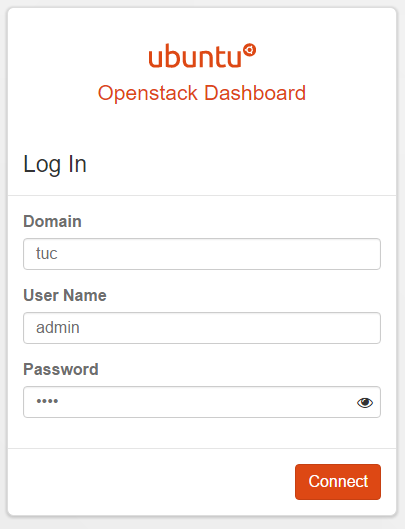
\includegraphics[width=0.7\linewidth]{dashboard_login}
  \caption{Login screen for the dashboard}\label{fig:dashboard_login}
\end{figure}
The dashboard can be accessed by using the web browser at: \\\verb|http://os-controller.etit.tu-chemnitz.de/horizon|.

Provide the login credentials to authenticate the user against the Keystone to login into the Dashboard.\\

The login credentials are:
\\Domain: \verb|TUC|
\\User Name: \verb|admin| or \verb|demo|
\\Password: user

The figure \ref{fig:network_topology_dashboard_view} shows the pictorial representation of the network and the instances created on the OpenStack under the link \textit{Network Topology}.

\begin{figure}[H]
  \centering
  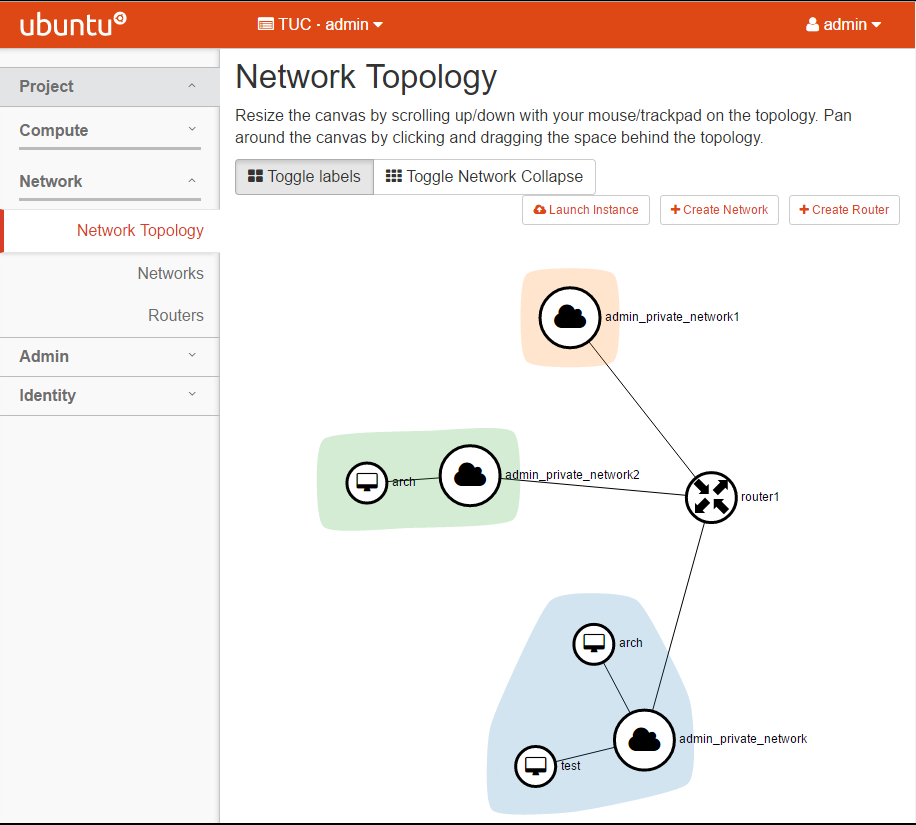
\includegraphics[width=1.0\linewidth]{network_topology_dashboard_view}
  \caption{The dashboard screen showing the diagrammatic representation of network topology}\label{fig:network_topology_dashboard_view}
\end{figure}

\subsection{Add the Telemetry service}\label{ssec:AddtheTelemetryservice}
The Object storage and Bloack storage services have not been deployed for the test bed.
The next service deployed is the OpenStack Telemetry service.

Telemetry service is deployed to have an analysis of metering data with respect to Compute and Image services.
Telemetry helps to efficiently poll the metering data related to OpenStack services.

Unlike other services, the Telemetry service uses a NoSQL database.
The MongoDB NoSQL server has been installed on the controller to be utilised by the Telemetry service.
The \verb|password| for the MongoDB is set to \verb|user|.

The ceilometer service entity and the API endpoints are created.
While configuring the endpoints for the Telemetry service, the \verb|region| is set to \verb|TUChemnitz|.
For example:
\begin{lstlisting}[frame=single]
$ openstack endpoint create --region TUChemnitz metering public http://controller:8777
\end{lstlisting}


The configuration of RabbitMQ message service needs some additional parameters that needs to be added in the \verb|/etc/ceilometer/ceilometer.conf| configuration file on the \verb|controller| node under the \verb|[oslo_messaging_rabbit]|.
\\Please refer to Appendix \nameref{app:sec:rabbitmq_config} for the \verb|[oslo_messaging_rabbit]| configuration parameters.
%\begin{lstlisting}[frame=single]
%[oslo_messaging_rabbit]
%rabbit_host = controller
%rabbit_port = 5672 #define ports
%rabbit_hosts = controller:5672
%rabbit_userid = openstack
%rabbit_password = user
%rabbit_use_ssl = false
%\end{lstlisting}

In the \verb|[service_credentials]| section, the \verb|os_region_name| is set as \verb|TUChemnitz|.
\begin{lstlisting}[frame=single]
[service_credentials]
...
os_region_name = TUChemnitz
\end{lstlisting}

Once the Telemetry service has been installed on \verb|controller|, it is configured to be consumed by Image service by editing the existing \verb|/etc/glance/glance-api.conf| and \verb|/etc/glance/glance-registry.conf| configuration files by adding the \\\verb|[oslo_messaging_rabbit]|.
\\Please refer to Appendix \nameref{app:sec:rabbitmq_config} for the \verb|[oslo_messaging_rabbit]| configuration parameters.

%\begin{lstlisting}[frame=single]
%[oslo_messaging_rabbit]
%rabbit_host = controller
%rabbit_port = 5672 #define ports
%rabbit_hosts = controller:5672
%rabbit_userid = openstack
%rabbit_password = user
%rabbit_use_ssl = false
%\end{lstlisting}

Once the OpenStack installation procedure with additional configuration as mentioned above is configured, the Telemetry is for Image service.

To enable the Telemetry service for Compute service, the ceilometer should be installed on each \verb|compute| node.
Once the Telemetry service has been installed on all the \verb|compute| nodes, it is configured to enable ceilometer by editing the \verb|/etc/ceilometer|-\verb|/ceilometer.conf| configuration file by adding the \verb|[oslo_messaging_rabbit]|.
Please refer to Appendix \nameref{app:sec:rabbitmq_config} for the \verb|[oslo_messaging_rabbit]| configuration parameters.

%\begin{lstlisting}[frame=single]
%[oslo_messaging_rabbit]
%rabbit_host = controller
%rabbit_port = 5672 #define ports
%rabbit_hosts = controller:5672
%rabbit_userid = openstack
%rabbit_password = user
%rabbit_use_ssl = false
%\end{lstlisting}

In the \verb|[service_credentials]| section, the \verb|os_region_name| is set as \verb|TUChemnitz|.
\begin{lstlisting}[frame=single]
[service_credentials]
...
os_region_name = TUChemnitz
\end{lstlisting}


\begin{figure}[H]
  \centering
  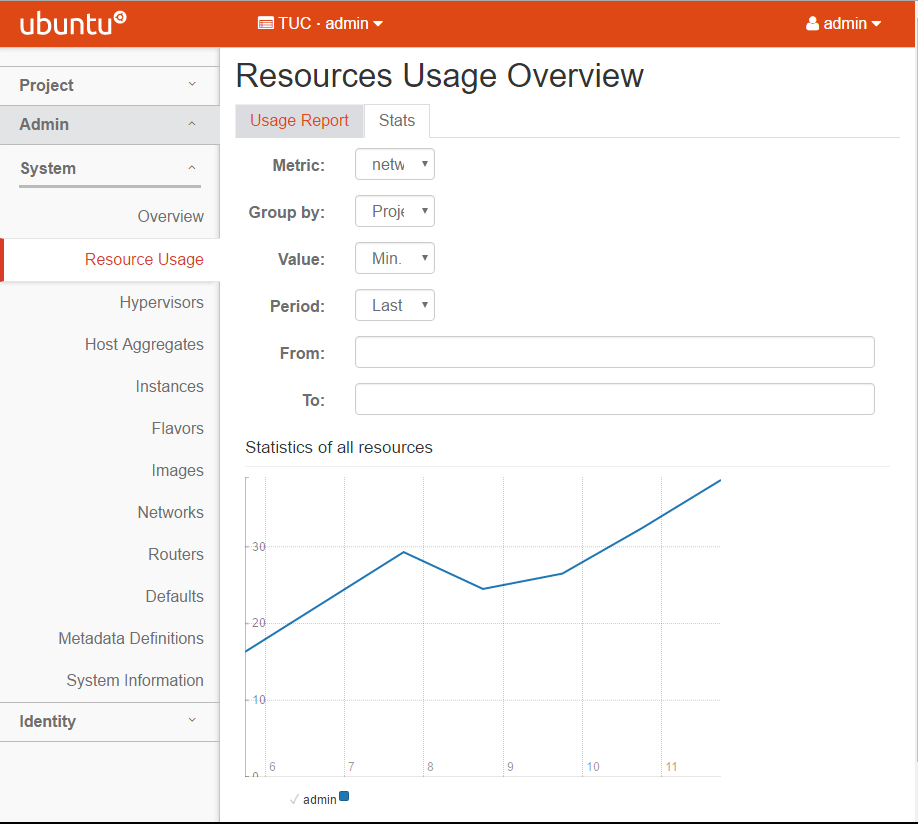
\includegraphics[width=1.0\linewidth]{telemetry_network_incoming_bytes}
  \caption{An example of the metering with the number of incoming bytes on a network for a virtual machine interface.}\label{fig:telemetry_network_incoming_bytes}
\end{figure}

All the above mentioned services have been installed and configured in the OpenStack test bed for this thesis.

%Das hier vorgestellte basiert auch dem Buch von~\cite{Heinkel2000}. Die Lösung kann auch mit einem \ac{fpga} sowie
%\ac{hw} und \ac{sw} entstehen.
%\blindtext[4]

%\subsection{Zweite Untergrundlage}\label{ssec:zweiteUGdl}

%\blindtext[1]
%\begin{table}[htpb]
%  \centering
%  \caption{Eine tolle Tabelle}\label{tab:ett}
%  \begin{tabular}{lcrl}
%  Links & Zentriert & Rechts & Links \\
%  \toprule
%  eins & zwei & drei & vier \\
%  eins & zwei & drei & vier \\
%  eins & zwei & drei & vier \\
%  \end{tabular}
%\end{table}

%Eine Tabelle benötigt auch eine Referenz, wie diese hier zu \ref{tab:ett}.
%\blindtext[1]

%\section{Zweite Grundlage}\label{sec:zweitegdl}

%\blindtext[2]

%\section{Dritte Grundlage}\label{sec:drittegdl}

%\blindtext[2]

% vim: ts=2:sw=2:sts=2:expandtab:wrapmargin=2:tw=120


% !TEX root       = ./type_name.tex
% !TEX program    = pdflatex
% !TEX encoding   = utf-8
% !TEX spellcheck = de_DE_frami
%=======================================================================

\chapter{Standard Nova Scheduling Algorithm}\label{ch:novaalgorithm}

OpenStack Nova uses the \verb|nova-scheduler| service to determine how to dispatch the compute requests which are requested by the user.
It calculates and determines on which \verb|compute| host node should the request for the virtual machine be processed.
The scheduler can be configured through a variety of options provided by the OpenStack.


\section{Theory of Nova Algorithm}\label{sec:novaalgorithmtheory}

As explained in \nameref{sec:novafilterschedulerdetailed}, the nova scheduler has a \textbf{Filter Scheduler} which supports the filtering and weighting the hosts to make informed decisions about on which host a new instance should or can possibly be created.

The filter scheduler iterates over each host and validates if the available resources on the host can support the requested virtual instance.
It creates a list of available hosts hosts which can serve the request to host an instance and proceeds with the filter mechanism.

The filter scheduler iterates over each available host, collects the resource information from the host and weighs according to the highest to lowest resource availability.

This filter scheduler in the Compute scheduler service is configured with the following default scheduler options in the \verb|/etc/nova/nova.conf| file:

\begin{lstlisting}[frame=single]
scheduler_driver_task_period = 60
scheduler_driver = nova.scheduler.filter_scheduler.FilterScheduler
scheduler_available_filters = nova.scheduler.filters.all_filters
scheduler_default_filters = RetryFilter, AvailabilityZoneFilter, RamFilter,DiskFilter, ComputeFilter, ComputeCapabilitiesFilter, ImagePropertiesFilter, ServerGroupAntiAffinityFilter, ServerGroupAffinityFilter
\end{lstlisting}

By default, the \verb|scheduler_driver| is configured with a filter scheduler which can be found at \verb|/usr/lib/python2.7/dist-packages/nova/scheduler/filter_sche|- \verb|duler.py| with the class name \verb|FilterScheduler|.

In the default configuration, this scheduler considers hosts that meet all the following criteria:

\begin{itemize}
	\item Any host that has not been attempted for scheduling purposes (RetryFilter).

	\item Any host that is available in the requested availability zone (AvailabilityZoneFilter).

	\item Any host that has sufficient availability of RAM to host an instance (RamFilter).

	\item Any host that has sufficient disk memory space available for root and ephemeral storage (DiskFilter).

	\item Any host that can and is available to service the request (ComputeFilter).

	\item Any host that can satisfy the extra specifications associated with the instance type (ComputeCapabilitiesFilter).

	\item Any host that can satisfy any architecture, hypervisor type, or virtual machine mode properties specified on the instance's image properties (ImagePropertiesFilter).

	\item Any host that is on a different host than other instances of a group (if requested) (ServerGroupAntiAffinityFilter).

	\item Any host that is in a set of group hosts (if requested) (ServerGroupAffinityFilter).

	\item Any host that is visible in the refreshed scheduler cache list of available hosts; by the use of \verb|scheduler_driver_task_period| option to specify how often the list is updated.
\end{itemize}

When the task of scheduling a virtual machine on a host is triggered by an user, the Filter Scheduler iterates over all found compute nodes, evaluating each against a set of filters.
The resultant list of available hosts are ordered by the weighers.

At the end, the Filter Scheduler sorts selected hosts by their weight and attempts to provision instances on the chosen hosts.

\newpage

\section{Code Trace}\label{sec:codetrace}

In this section, the code trace to the nova scheduler can be observed.

When an instance is requested, it is received by the nova API listener for validation of the nova API URL and processes the requested tasks based on the requested input parameters.
The Nova API reads the default scheduler file from the \verb|/etc/|\verb|nova/| \verb|nova.conf| file.
In the python source file \verb|filter_scheduler|, the \verb|FilterScheduler| \verb|class| is initialized by the \verb|driver.Scheduler| driver.

The scheduler driver object calls the \verb|def| \verb|select_destinations(self,| \verb|context,| \verb|request_spec,| \verb|filter_properties)| function in the \verb|FilterScheduler| class.
\newline
\begin{lstlisting}[frame=single, language=Python, caption={The function select\_destination},label={lst:select_destinations}, escapechar=|]
def select_destinations(self, context, request_spec, filter_properties):
	"""Selects a filtered set of hosts and nodes."""
	self.notifier.info(context,
		'scheduler.select_destinations.start',
		dict(request_spec=request_spec))

	# Count of requested virtual instances
	num_instances = request_spec['num_instances']

	# The FilterScheduler._schedule function is called,
	# which schedules the possible hosts for the requested instances
	selected_hosts = self._schedule(context, request_spec,|\label{line:select_destinations_schedule}|
		filter_properties)

	...
	...
	
\end{lstlisting}

In the above code listing \ref{lst:select_destinations}, the function \verb|_schedule| called at line \ref{line:select_destinations_schedule}
initiates the scheduling algorithm by passing the \verb|request_spec| as the parameter which holds all the specifications for creating the virtual instances like; requested number of instances, required RAM capacity per instance, required HDD capacity per instance, required VCPUs per instance, required OS image to boot the virtual instance with it, and other instance related parameters.

Stepping into the function \verb|FilterScheduler._schedule| given in listing \ref{lst:select_destinations_schedule}.
\newline
\begin{lstlisting}[frame=single, language=Python, caption={The function \_schedule}, label={lst:select_destinations_schedule}, escapechar=|]
def _schedule(self, context, request_spec, filter_properties):
	"""Returns a list of hosts that meet the required specs,
	ordered by their fitness.
	"""

	...
	...
	
	# iterate each host and select the host to place an instance
	for num in range(num_instances):
		# Filter local hosts based on requirements ...
		hosts = self.host_manager.get_filtered_hosts(hosts,|\label{line:get_filtered_hosts}|
				filter_properties, index=num)
		if not hosts:
			# Can't get any more locally.
			break

		LOG.debug("Filtered %(hosts)s", {'hosts': hosts})

		# weigh the hosts based on the weighing filter
		weighed_hosts = self.host_manager.get_weighed_hosts(hosts,|\label{line:get_weighed_hosts}|
				filter_properties)

		...
		...
		
		chosen_host = random.choice(
			weighed_hosts[0:scheduler_host_subset_size])
		LOG.debug("Selected host: %(host)s", {'host': chosen_host})
		selected_hosts.append(chosen_host)|\label{line:chosen_host}|

		...
		...

	LOG.info('%s number of instances scheduled with filter scheduler in %s seconds' % (num_instances, (rtime.time() - start_time)))
	return selected_hosts
\end{lstlisting}


In the listing \ref{lst:select_destinations_schedule}, at the line number \ref{line:get_filtered_hosts}, the function \verb|get_filtered_hosts| in the class \verb|HostManager| in the python source file \verb|host_manager| is called to filter the hosts based on the RAM filter, Disk Filter, Compute Filter, and other specified filters in the list.

Stepping into the \verb|get_filtered_hosts| given in listing \ref{lst:get_filtered_hosts}.
\newline
\begin{lstlisting}[frame=single, language=Python, caption={The function get\_filtered\_hosts}, label={lst:get_filtered_hosts}, escapechar=|]
def get_filtered_hosts(self, hosts, filter_properties,
		filter_class_names=None, index=0):
	"""Filter hosts and return only ones passing all filters."""

	...
	...
	
	if filter_class_names is None:
		filters = self.default_filters|\label{line:default_filters}|
	else:
		filters = self._choose_host_filters(filter_class_names)|\label{line:choose_host_filters}|
	ignore_hosts = filter_properties.get('ignore_hosts', [])
	force_hosts = filter_properties.get('force_hosts', [])
	force_nodes = filter_properties.get('force_nodes', [])

	...
	...
	return self.filter_handler.get_filtered_objects(filters,
			hosts, filter_properties, index)
\end{lstlisting}

In this listing \ref{lst:get_filtered_hosts}, the filter classes are loaded either by default at line number \ref{line:default_filters} or by the specified list of filters at line number \ref{line:choose_host_filters}.
These classes include the \verb|nova|.\verb|scheduler|. \verb|filters|.\verb|ram_filter|, \verb|nova|.\verb|scheduler|.\verb|filters|.\verb|disk_filter|, \verb|nova|.\verb|scheduler|.\newline\verb|filters|.\verb|compute_filter| and other specified default filters.

In the listing \ref{lst:select_destinations_schedule}, at the line number \ref{line:get_weighed_hosts}, the function \verb|get_weighed_hosts| in the class \verb|HostManager| in the python source file \verb|host_manager| is called to get list of hosts sorted according to the weights calculated by the weights filter. At line \ref{line:chosen_host} the chosen host is then set as selected host for the requested virtual instance.

The listing \ref{lst:get_weighed_hosts} calculates the weights of each host by comparing with the available properties of host and the requested properties of an instance as mentioned in the section \ref{ssec:novaweights}
\begin{lstlisting}[frame=single, language=Python, caption={The function \_schedule}, label={lst:get_weighed_hosts}, escapechar=|]
def get_weighed_hosts(self, hosts, weight_properties):
	"""Weigh the hosts."""
	return self.weight_handler.get_weighed_objects(self.weighers,
			hosts, weight_properties)
\end{lstlisting}

The \verb|get_weighed_objects| looks for actual available resources on the hosts and calculates the weight of each objects.

The custom trace of the log can be observed in the Appendix \nameref{app:ch:logs} at \nameref{app:sec:filterschedulerlogtrace}.
% !TEX root       = ./type_name.tex
% !TEX program    = pdflatex
% !TEX encoding   = utf-8
% !TEX spellcheck = de_DE_frami
%=======================================================================

\chapter{Implementation of Cplex based Nova Scheduler}\label{ch:implementationofcplex}

After the iterations of debugging the OpenStack Scheduler Python module, the key parameters which contribute in the calculation of the placement decisions of virtual instances are identified.
The key parameters that would be required in computation of placements decision are:
\begin{itemize}
	\item Available RAM capacity on each of the Compute node and
	\item Available Hard Disk capacity on each of the Compute node
\end{itemize}

The number of CPU cores are not taken into consideration.
As the Compute nodes support the hardware acceleration for virtual machines using the KVM mode, the CPU cores can be over utilised.
The default \verb|cpu_allocation_ratio| is set to 16 which allows the over creation of virtual CPU cores, due to which the available CPU cores do not play a major role in determining the creation of virtual instances.

In this chapter, the formulation of the new cPlex based Mathematical model is explained,
and also the implemented code is provided with an explanation.

\section{Mathematical Formulation}\label{sec:mathematicalformulation}
The idea behind the mathematical formulation is to implement the energy efficient scheduler mechanism, where the placement decisions are made to utilise maximum capacity of the Compute node before a new placement decision is requested on the other Compute nodes. This was conceptualised with an idea to extend the algorithm with an ability to perform live migration of the existing virtual machines to re-order the placement decisions.

As the live migration is still a work in progress, the mathematical model is formulated with only the essential parameters into considerations.

Parameters for the mathematical model are defined as follows:
\\$n_s$ is the host number in the set of nodes.
\\$N_s$ is the set of all the host nodes.
\\$n_v$ is the virtual instance number in the requested virtual instances list.
\\$N_v$ is the set of all the requested virtual instances to be placed.
\\$x_{n_s}$ is the each individual host node.
\\$x_{n_s}^{n_v}$ is the unique combination of requested virtual instance from the set of $N_v$ and host node from the set of $N_s$.
\\$suit_{n_s}^{n_v}$ is the suitable host entry for the requested virtual instance.
\\$d_{n_v}^{RAM}$ is the required demand of RAM for the given virtual instance.
\\$c_{n_s}^{RAM}$ is the available capacity of RAM in the given host node.
\\$d_{n_v}^{HDD}$ is the required demand of hard disk for the given virtual instance.
\\$c_{n_s}^{HDD}$ is the available capacity of hard disk in the given host node.

The objective function is to minimize the host nodes for placing the requested virtual instances. 
This objective function can be given as:
\begin{equation} \label{eq:1}
\min{\sum_{n_s \in N_s}{x_{n_s}}}
\end{equation}

For each virtual instance, the placement request of the virtual instance is done on one and only one host node. This can be given by the equation:
\begin{equation} \label{eq:2}
\sum_{n_s \in N_s}{x_{n_s}^{n_v}}{suit_{n_s}^{n_v}} = 1, \forall{n_v} \in N_v
\end{equation}

The equation to determine if the host is suitable or not suitable for a given combination of virtual instance and host is given by:
\begin{equation} \label{eq:3}
x_{n_s}^{n_v} \leq suit_{n_s}^{n_v},\forall{n_s} \in N_s, n_v \in N_v
\end{equation}

The equation which evaluates if the placement decision can be made on the given host node or not for a given virtual instance is given by:
\begin{equation} \label{eq:4}
x_{n_s} \geq x_{n_s}^{n_v},\forall{n_s} \in N_s, n_v \in N_v
\end{equation}

The RAM capacity constraints are given as follows:
\begin{equation} \label{eq:5}
\sum_{n_v \in N_v}{x_{n s}^{n_v}}{d_{n_v}^{RAM}} \leq c_{n_s}^{RAM}, \forall{n_s} \in N_s 
\end{equation}

The hard disk(HDD) capacity constraints are given as follows:
\begin{equation} \label{eq:6}
\sum_{n_v \in N_v}{x_{n s}^{n_v}}{d_{n_v}^{HDD}} \leq c_{n_s}^{HDD}, \forall{n_s} \in N_s 
\end{equation}

These equations provide the boundary conditions to determine the possible placement decision of the virtual instances in the host nodes.

\section{The overview of implementation}\label{sec:overviewofimplementation}

IBM ILOG CPLEX\textsuperscript{\textregistered} Optimizer is a mathematical programming technology that enables decision of mathematical optimization for improving efficiency, reducing costs, and increasing profitability\cite{cplex-optimizer}.
This software is used to provide the solution for placement decision of the virtual instances on the host nodes.
For the purpose of this Thesis, the version 12.6 of the IBM Cplex is used.

To implement the mathematical formulation described in the section \nameref{sec:mathematicalformulation}, a new scheduler file is created with a name \verb|"tuc_ccn_scheduler.py"|.

The \verb|tuc_ccn_scheduler.py| has the class and function definition similar to the default \verb|FilterScheduler|.
There are few changes in the implementation of the \verb|_schedule| function and a new function named as \verb|solve_TUC_Cplex| has been added to implement the new cPlex based mathematical scheduling model.

The \verb|_schedule| function for the new \verb|tuc_ccn_scheduler| is given as:
\newline
\begin{lstlisting}[frame=single, language=Python, caption={The cPlex based TUC\_scheduler's \_schedule function}, label={lst:tuc_schedule}, escapechar=|]
def _schedule(self, context, request_spec, filter_properties):
	"""Returns a list of hosts that meet the required specs,
	ordered by their fitness.
	"""
	elevated = context.elevated()
	instance_properties = request_spec['instance_properties']

	# NOTE(danms): Instance here is still a dict, which is converted from
	# an object. The pci_requests are a dict as well. Convert this when
	# we get an object all the way to this path.
	# TODO(sbauza): Will be fixed later by the RequestSpec object
	pci_requests = instance_properties.get('pci_requests')
	if pci_requests:
		pci_requests = (
			objects.InstancePCIRequests.from_request_spec_instance_props(
				pci_requests))
		instance_properties['pci_requests'] = pci_requests

	instance_type = request_spec.get("instance_type", None)

	update_group_hosts = filter_properties.get('group_updated', False)

	config_options = self._get_configuration_options()

	filter_properties.update({'context': context,
							  'request_spec': request_spec,
							  'config_options': config_options,
							  'instance_type': instance_type})

	# Find our local list of acceptable hosts by repeatedly
	# filtering and weighing our options. Each time we choose a
	# host, we virtually consume resources on it so subsequent
	# selections can adjust accordingly.

	# Note: remember, we are using an iterator here. So only
	# traverse this list once. This can bite you if the hosts
	# are being scanned in a filter or weighing function.
	hosts = self._get_all_host_states(elevated)
	selected_hosts = []
	num_instances = request_spec.get('num_instances', 1)

	# the function get_filtered_hosts is called only once
	# before the for loop unlike the default scheduler's
	# _schedule function
	hosts = self.host_manager.get_filtered_hosts(hosts,|\label{line:tuc_get_filtered_hosts}|
			filter_properties, index=0)

	weighed_hosts = self.weight_handler.get_weighed_objects(self.weighers,
			hosts, filter_properties)

	vi_hosts = {}
	start_time = rtime.time()
	# implementation of cPlex based mathematical solver
	try:
		vi_hosts = self.solve_TUC_Cplex(hosts, filter_properties, num_instances)|\label{line:solve_TUC_Cplex}|
	except CplexError as exc:
		LOG.error('%s', exc)
		reason = _(exc)
		raise exception.NoValidHost(reason=reason)
	#end of the function call within try and exception
	
	for num in range(num_instances):
		weighed_hosts = vi_hosts[num]

		scheduler_host_subset_size = CONF.scheduler_host_subset_size

		if scheduler_host_subset_size > len(weighed_hosts):
			scheduler_host_subset_size = len(weighed_hosts)
		if scheduler_host_subset_size < 1:
			scheduler_host_subset_size = 1

		chosen_host = weighed_hosts[0]
		LOG.debug("Selected host: %(host)s", {'host': chosen_host})

		# append the selected hosts  to the array mapping
		selected_hosts.append(chosen_host)

		# Now consume the resources so the filter/weights
		# will change for the next instance.
		chosen_host.obj.consume_from_instance(instance_properties)
		if update_group_hosts is True:
			# NOTE(sbauza): Group details are serialized into a list now
			# that they are populated by the conductor, we need to
			# deserialize them
			if isinstance(filter_properties['group_hosts'], list):
				filter_properties['group_hosts'] = set(
					filter_properties['group_hosts'])
			filter_properties['group_hosts'].add(chosen_host.obj.host)
	LOG.info('%s number of instances scheduled with tuc scheduler in %s seconds' % (num_instances, (rtime.time() - start_time)))
	return selected_hosts
\end{lstlisting}

In the above code listing \ref{lst:tuc_schedule}, the \verb|get_filtered_hosts| at line number \ref{line:tuc_get_filtered_hosts} is called before the for loop and called only once to provide an input to cPlex solver, unlike the default scheduler which filters the hosts for each request of an instance.

The cPlex based solver funtion is called at line number \ref{line:solve_TUC_Cplex}. The hosts, filter\_properties and num\_instances are passed as parameters to the function in the listing \ref{lst:solve_TUC_Cplex}.
\newline
\begin{lstlisting}[frame=single, language=Python, caption={The cPlex based TUC\_scheduler's solve\_TUC\_Cplex function}, label={lst:solve_TUC_Cplex}, escapechar=|]
def solve_TUC_Cplex(self, hosts, filter_properties, num_instances):
	weighedHosts    = []
	#available RAM capacity on each compute (host) node
	ns_rams         = []
	#available HDD capacity on each compute (host) node
	ns_hdds         = []
	for host in hosts:
		weighedHost = []
		weighedHost.append(host)
		weighedHost = self.host_manager.get_weighed_hosts(weighedHost,
				filter_properties)
		weighedHosts.append(weighedHost)
		ns_rams.append(host.free_ram_mb)
		ns_hdds.append(host.free_disk_mb)

	instance_type = filter_properties['instance_type']
	root_gb     = instance_type['root_gb']
	memory_mb   = instance_type['memory_mb']
	nvram       = 1.0*memory_mb
	nvhdd       = 1024.0*root_gb
	my_prob     = cplex.Cplex()

	#Number of hosts available to cater the requested instances
	host_count  = len(hosts)
	vis         = num_instances

	# cPlex input parameters
	# objective function parameters
	my_obj      = []
	# upper bound values
	my_ub       = []
	# lower bound values
	my_lb       = []
	# parameter type
	my_ctype    = ''
	# names of all the mathematical parameters
	my_colnames = []
	# the values on the right hand side
	my_rhs      = []
	# unique name for each row
	my_rownames = []
	my_sense    = ''

	rows        =   []

	# translate the mathematical formulations into cPlex input
	for i in range(host_count):
		my_obj.append(1.0)
		my_colnames.append("x_"+str(i))
		my_ub.append(1.0)
		my_lb.append(0.0)
		my_ctype = my_ctype+'B'
		vvar  = []
		vvalr = []
		vvalh = []
		for j in range(vis):
			my_obj.append(0.0)
			my_colnames.append("x_"+str(i)+"_"+str(j))
			my_ub.append(1.0)
			my_rhs.append(0.0)
			my_ctype = my_ctype+'B'
			my_lb.append(0.0)
			row = []
			var = []
			val = []
			var.append("x_"+str(i))
			var.append("x_"+str(i)+"_"+str(j))
			val.append(1.0)
			val.append(-1.0)
			row.append(var)
			row.append(val)
			rows.append(row)
			my_rownames.append('rsv_'+str(i)+'_'+str(j))
			my_sense = my_sense+'G'
			vvar.append("x_"+str(i)+"_"+str(j))
			vvalr.append(nvram)
			vvalh.append(nvhdd)
		row = []
		row.append(vvar)
		row.append(vvalr)
		rows.append(row)
		my_rhs.append(ns_rams[i])
		my_sense = my_sense+'L'
		my_rownames.append('rsram_'+str(i))
		row = []
		row.append(vvar)
		row.append(vvalh)
		rows.append(row)
		my_rhs.append(ns_hdds[i])
		my_sense = my_sense+'L'
		my_rownames.append('rshdd_'+str(i))

	for i in range(vis):
		row = []
		var = []
		val = []
		for j in range(host_count):
			var.append("x_"+str(j)+"_"+str(i))
			val.append(1.0)
		my_sense = my_sense+'E'
		row.append(var)
		row.append(val)
		rows.append(row)
		my_rhs.append(1.0)
		my_rownames.append('rnv_'+str(i))

	my_prob.objective.set_sense(my_prob.objective.sense.minimize)

	my_prob.variables.add(obj=my_obj, lb=my_lb, ub=my_ub,
		types=my_ctype, names=my_colnames)

	# pass all parameters to cPlex to solve the equation
	my_prob.linear_constraints.add(lin_expr=rows, senses=my_sense,
		rhs=my_rhs, names=my_rownames)
	# solve the mathematical model
	my_prob.solve()

	numcols = my_prob.variables.get_num()
	numrows = my_prob.linear_constraints.get_num()

	slack = my_prob.solution.get_linear_slacks()
	# get the solution values
	x = my_prob.solution.get_values()

	vi_hosts = {}
	for i in range(vis):
		for j in range(host_count):
			vi_host = (j*vis+1+j)+i
			if x[vi_host] == 1.0:
				vi_hosts[i] = weighedHosts[j]

	#LOG.info('VI Hosts: %(vih)s', {'vih': vi_hosts})
	return vi_hosts
\end{lstlisting}

The above code listing \ref{lst:solve_TUC_Cplex} is a cPlex based approach to perform scheduling of virtual instances.

The comparisions of both the schedulers and their performances are provided in the chapter \nameref{ch:comparisionofbothscheduler}.

% !TEX root       = ./type_name.tex
% !TEX program    = pdflatex
% !TEX encoding   = utf-8
% !TEX spellcheck = de_DE_frami
%=======================================================================

\chapter{Comparision of performance evaluation}\label{ch:comparisionofbothscheduler}

In this chapter, observations are made based on both the schedulers.
The data based on default nova scheduler driver and the data based on tuc\_scheduler driver are evaluated for different iterations of scheduling of virtual instances.
A data set of different number of virtual instance creation is performed on both of the scheduler drivers.



\section{Observations of standard Nova scheduler}\label{sec:observationsofstandardnova}

Observing the listing \ref{lst:select_destinations_schedule}, at the line \ref{line:get_filtered_hosts} it can be seen that the \verb|get_filtered_hosts| is performed for each virtual instance scheduling rather than once for the whole of the request. This is also followed by line \ref{line:get_weighed_hosts} to get weighed hosts for each virtual instance scheduling instead of once for the whole of the request.

In the log trace listing \ref{lst:filterschedulercodetracelog10vi} at the line number \ref{line:result_filter_scheduler_placement}, it can be observed that, the placement decision of the 10 virtual instances is spread across all the host systems.
This creates the need to keep the hosts powered up for all the time.

The log trace listing \ref{lst:filterschedulercodetracelog10vi} provided in the Appendix \nameref{app:ch:logs} in chapter \nameref{app:sec:filterschedulerlogtrace10vi} shows the number of times the \verb|get_filtered-| \verb|_hosts| and \verb|get_weighed_hosts| is called to calculate the placement decision of 10 virtual instances.

\begin{figure}[H]
	\begin{center}
		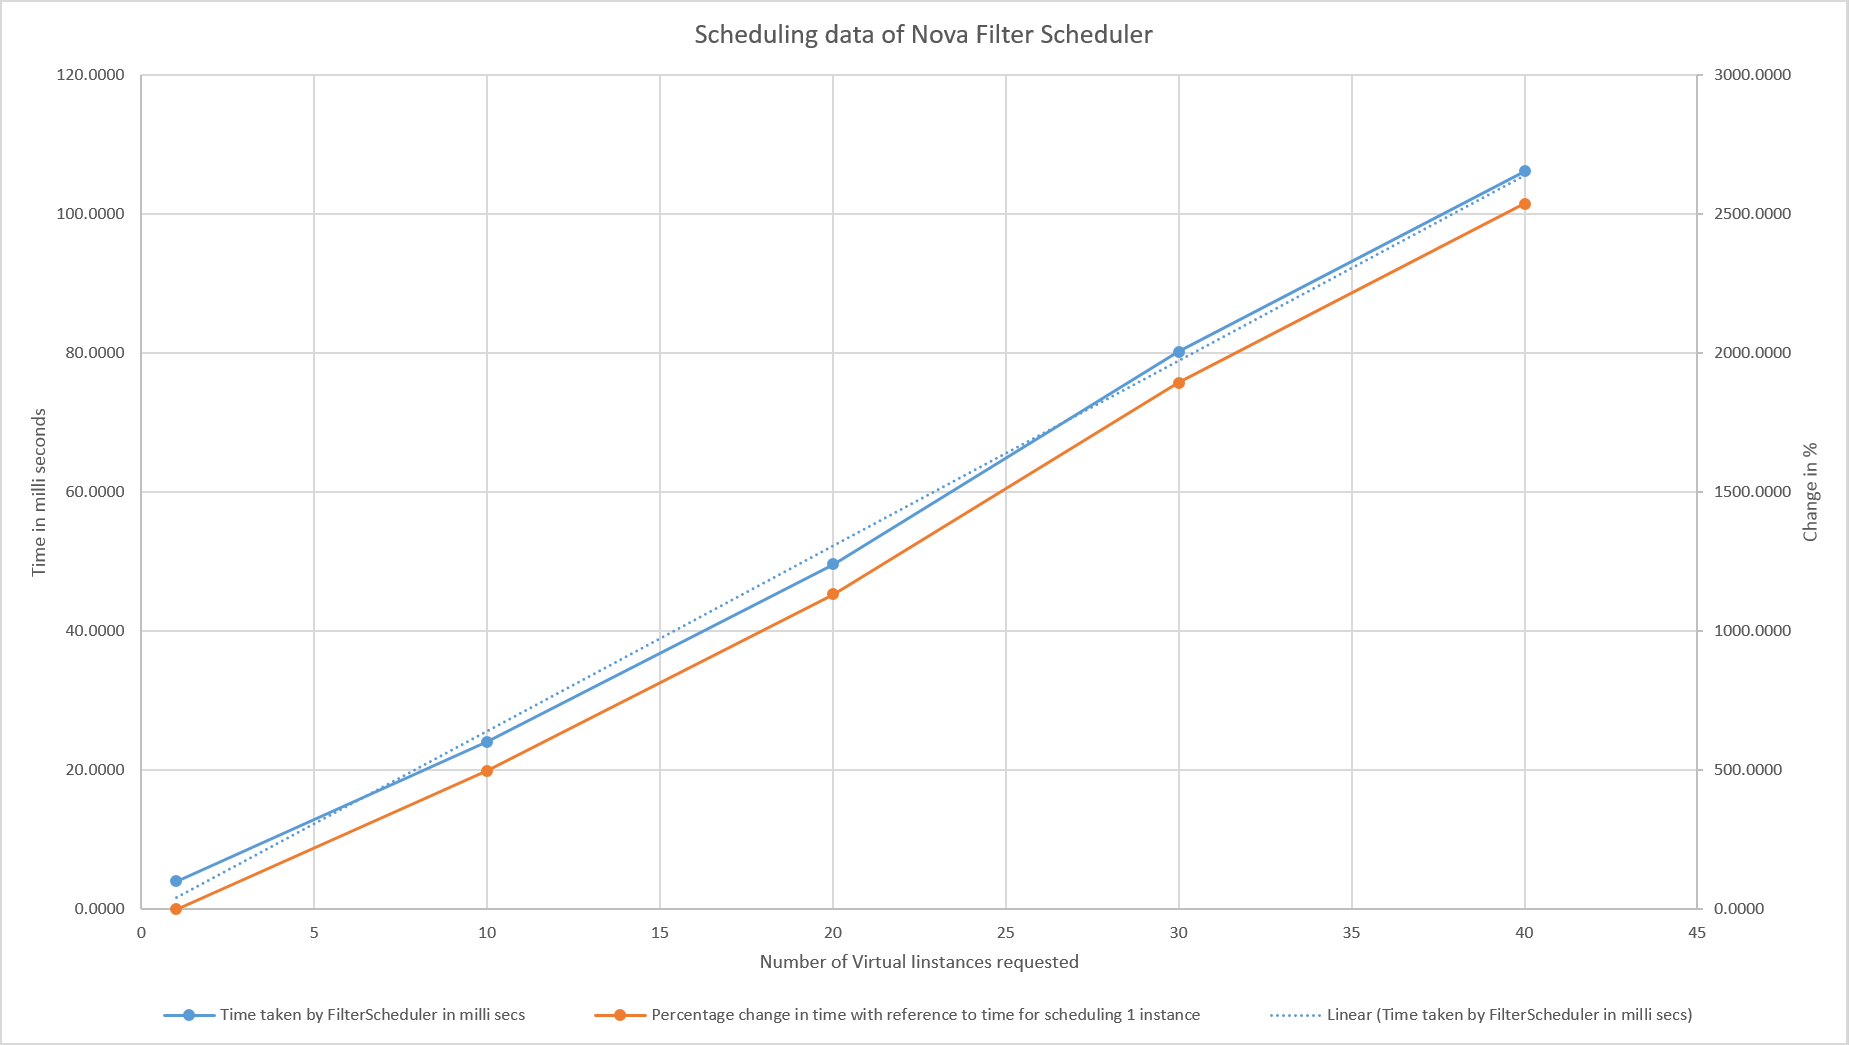
\includegraphics[width=1\linewidth]{NovaFilterSchedulerChart}
		\caption{Placement decision time for Standard Nova Scheduler from the data \ref{tabular:filterschedulerlogdata}}
		\label{fig:NovaFilterSchedulerChart}
	\end{center}
	\vspace{-10pt}
\end{figure}

The above table \ref{tabular:filterschedulerlogdata} is the time logs recorded for different requested number of virtual instances.
Here in the table, for providing a placement decision of 10 virtual instances, the standard nova scheduler takes around 24.10ms.
The percentage change in time is given by the change in time with reference to time for scheduling 1 instance.

\section{Observations of cPlex based scheduler}\label{sec:observationsoftucscheduler}

Observing the listing \ref{lst:tuc_schedule}, at the line \ref{line:tuc_get_filtered_hosts} it can be seen that the \verb|get_filtered_hosts| is executed only once for all the bulk requests of virtual instance scheduling.
This is followed by line \ref{line:solve_TUC_Cplex} \verb|solve_TUC_Cplex| to solve the scheduling problem for all the bulk requests.

In the log trace listing \ref{lst:tucschedulercodetracelog10vi} at the line number \ref{line:result_cplex_scheduler_placement}, it can be observed that, the placement decision of all the 10 virtual instances is concentrated on one host system \verb|"compute03"|.

The log trace listing \ref{lst:tucschedulercodetracelog10vi} provided in the Appendix \nameref{app:ch:logs} in chapter \nameref{app:sec:cplexschedulerlogtrace10vi} shows that only one instance of the \verb|get_filtered_hosts| is called to calculate the placement decision of 10 virtual instances.

\begin{figure}[H]
	\begin{center}
		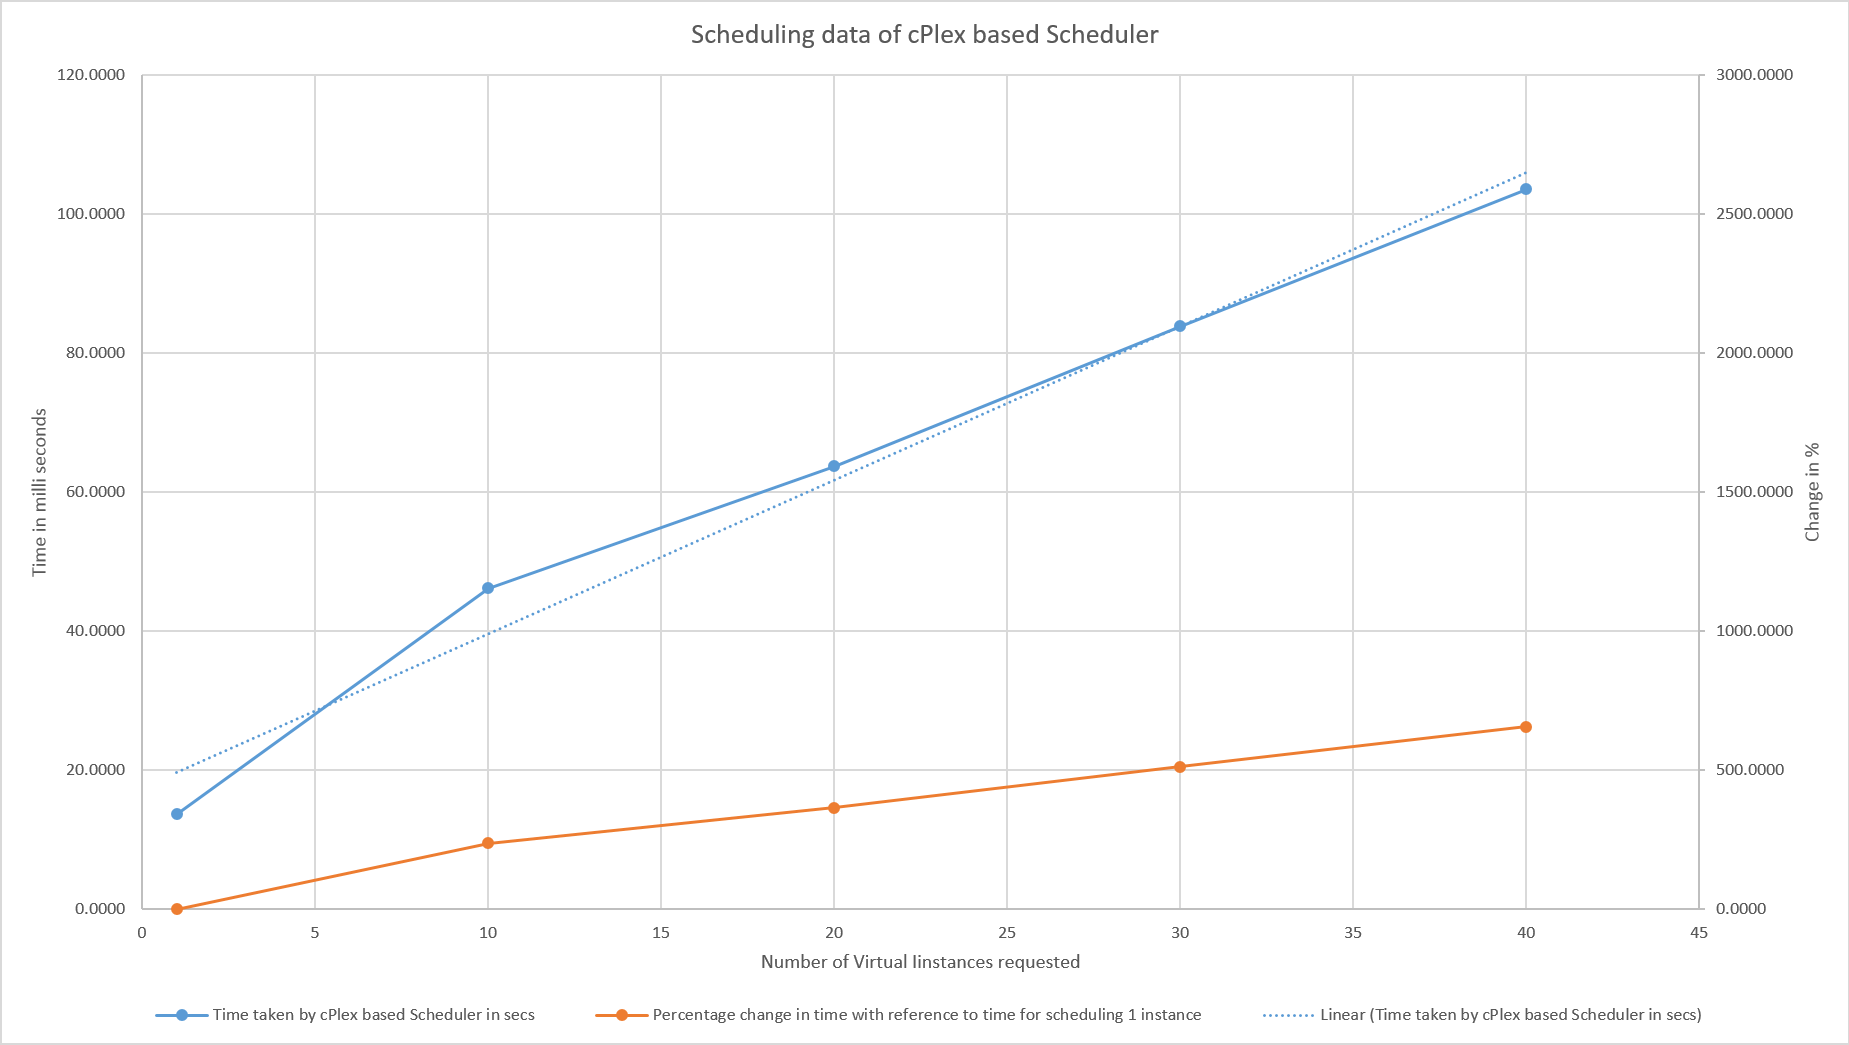
\includegraphics[width=1\linewidth]{cPlexSchedulerChart}
		\caption{Placement decision time for cPlex based Scheduler from the data \ref{tab:tucschedulerlogdata}}
		\label{fig:cPlexSchedulerChart}
	\end{center}
	\vspace{-10pt}
\end{figure}

\comment{
If the total requested capacity of RAM or HDD of virtual instances are more than the total available capacities, then the cPlex throws an exception as "unsolvable problem error". This exception is caught by the code and displayed as an error message on the screen.
}
\section{Comparision}\label{sec:comparision}

As stated in sections \nameref{sec:observationsofstandardnova} and \nameref{sec:observationsoftucscheduler}, the default Filter scheduler places the virtual instances across the hosts, whereas the \verb|tuc_ccn_scheduler| aggregates the creation of virtual instances on minimum possible host systems.
As the virtual instances on the new \verb|tuc_ccn_scheduler| are not spread across the multiple machines and aggregated on the few machines, the rest of the machines can be powered down which reduces the operating power costs.

On the other hand, combining the above two charts \ref{fig:NovaFilterSchedulerChart} and \ref{fig:cPlexSchedulerChart}, it can be observed that the slope of the cplex based scheduler is lesser than the slope of the standard nova filter scheduler. Which means that, for a larger requests of virtual instances, the cPlex based scheduler would be more efficient in providing the placement decisions for all the requested virtual instances. The initial offset time for execution of cPlex to solve the mathematical problem is higher compared to the standard nova filter scheduler.

\begin{figure}[H]
	\begin{center}
		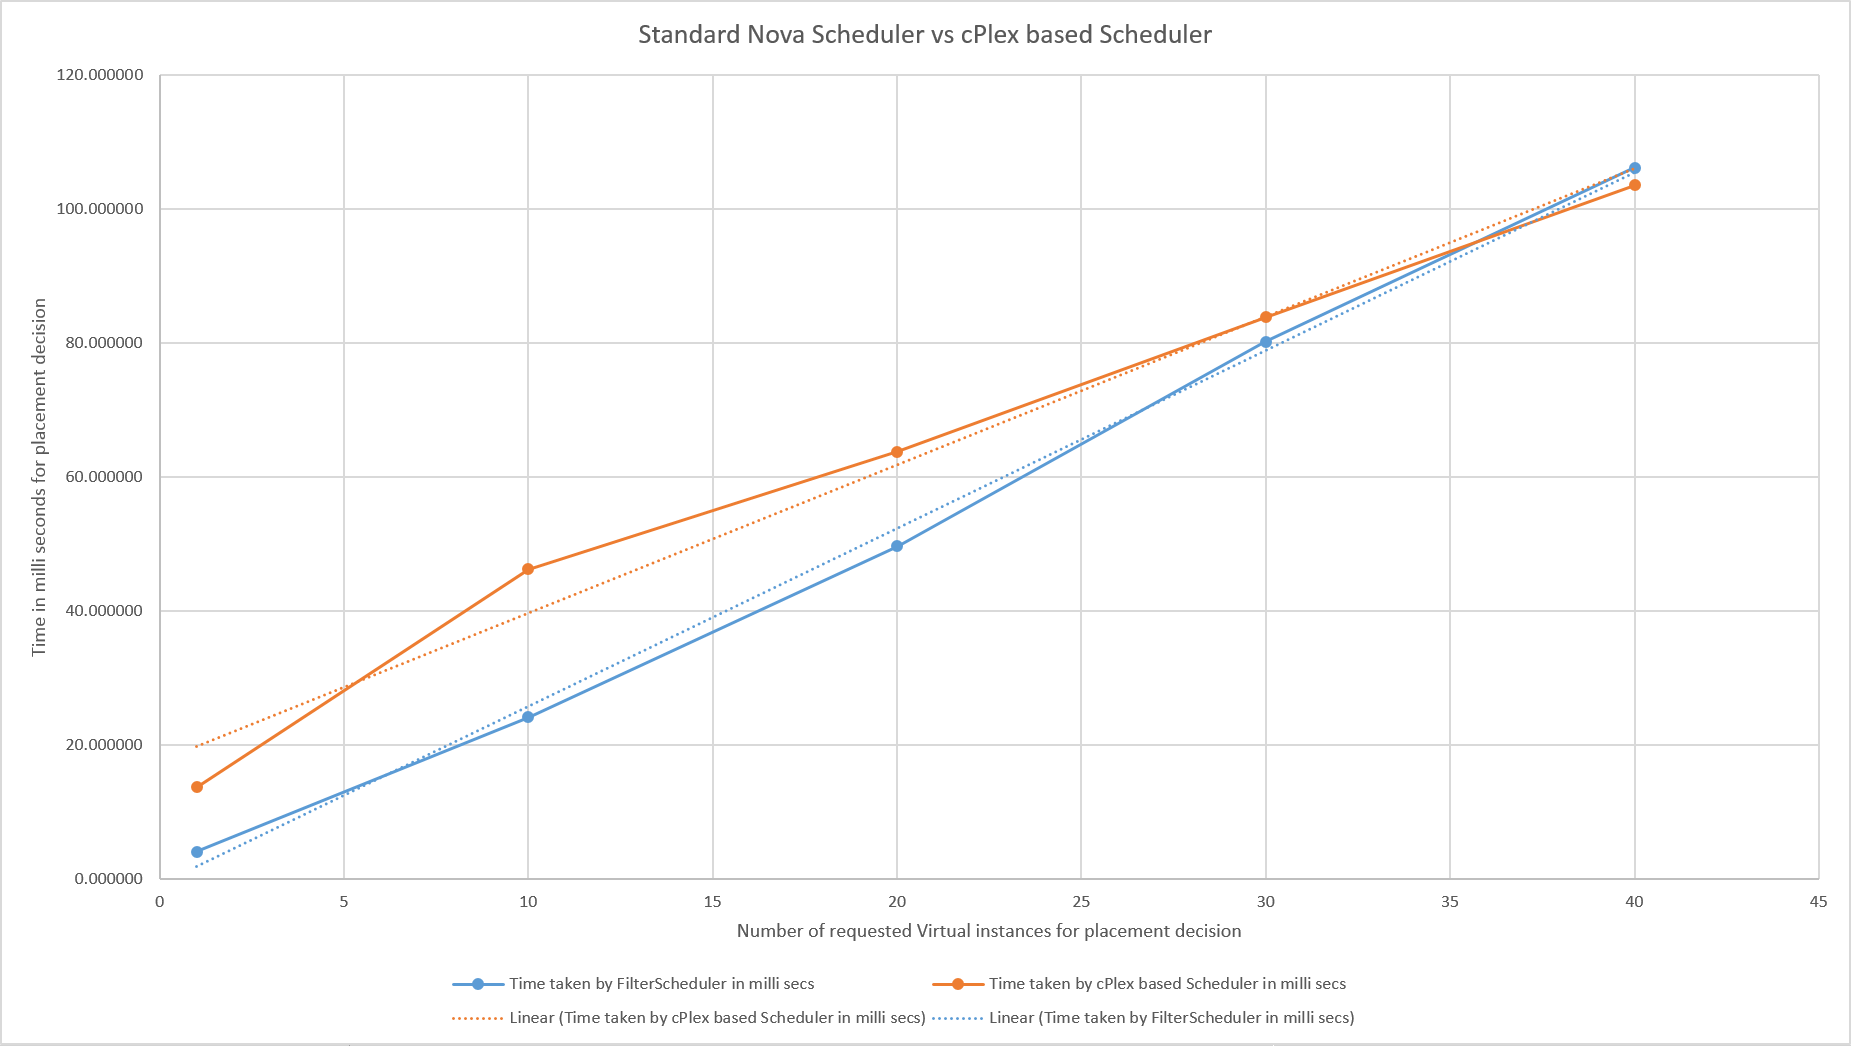
\includegraphics[width=1\linewidth]{novavscplex}
		\caption{Comparision of placement decision time between Standard Nova FilterScheduler and cPlex based Scheduler}
		\label{fig:novavscplex}
	\end{center}
	\vspace{-10pt}
\end{figure}

From the above chart \ref{fig:novavscplex}, it can be concluded that, the higher the number of requests to schedule the virtual instances the lesser the solving time for scheduling compared to the nova filter scheduler.

\section{Space for further improvements}\label{sec:spaceforimprovements}

As an example, let there be three host machines with a RAM capacity of 16GB each.
Let there be 9 virtual machines which consume 4GB of RAM each and shared equally among three host machines.
The available capacity of RAM is limited to 4GB on each machine whereas the total available capacity of RAM across all the machines is 12GB.
When there is a request for a virtual machine which requires the RAM of 8GB, both the schedulers would fail to make a placement decision for the requested virtual instance as there is no host with an available capacity of 8GB.

"Live Migration" is a functionality which would move the running virtual machine from one physical host machine to another physical host machine with minimum or no downtime.
Currently, the OpenStack Liberty has an ongoing issue with "Live Migration".
The live migration functionality fails to migrate the virtual instance from the source host machine to requested destination host machine and turns off the virtual instance scheduled for migration.
This "Live Migration" functionlity could mitigate the above mentioned issue with runtime reallocation of live(running) virtual machines to free the space by migrating it to any other possible hosts, freeing the space on the host and make a placement decision to allocate a new request of 8GB.

An idea for future could also be to have a shared resource pooling with a high speed dedicated networking bus on the hardware, to make the large clusters of compute servers into a single shared entity.
% !TEX root       = ./type_name.tex
% !TEX program    = pdflatex
% !TEX encoding   = utf-8
% !TEX spellcheck = de_DE_frami
%=======================================================================

\chapter{Further possible extensions in OpenStack}\label{ch:futurepossibilities}
Being one of the key open source software platform for Cloud Computing in Infrastructure-as-a-Service model, it has various possible implementations and extensions.
As far as networking is concerned, there are modules in and out of OpenStack which provides the Network Functions Virtualization (NFV) for global telecom providers.

Network Functions Virtualization (NFV) allows telecom and enterprise network operators to control their networking functions: physical, virtual and functional domains—using commercial off-the-shelf hardware, and open source software as a single control pane for management and orchestration.
Here, OpenStack can provide a platform for the development and evolution of NFV components across the virtual systems. With robust system level integration and deployment a reference NFV platform can be created to accelerate the transformation of enterprise and service provider networks.

Early on, the telecommunications industries and the networking vendors have recognised the potential for OpenStack as a platform for NFV, which triggered investigations and work in development of OpenStack compatible modules to optimize for NFV.

"Network Functions Virtualization (NFV) is now synonymous with OpenStack. When people say NFV, there is an implication that they are talking about OpenStack."\cite{openstack_nfv}

Both the European Telecommunications Standards Institute and Linux Foundation collaboration project OPNFV have defined specifications and released reference platforms for NFV that select OpenStack as the Virtualization Infrastructure Manager. Additionally, OpenStack is the dominant choice for additional management and orchestration functions.\cite{nfv_technical_overview}

The interoperability between OpenStack and virtualized network functions is still an ongoing development.

So, what does Network Functions Virtualization (NFV) define?
To answer in a simple way, it is a new way to define, create, and manage networks by replacing dedicated network appliances with software and automation.
It is the idea of replacing the physical network devices which are dedicated and expensive by the virtual software devices.

\begin{figure}[H]
	\begin{center}
		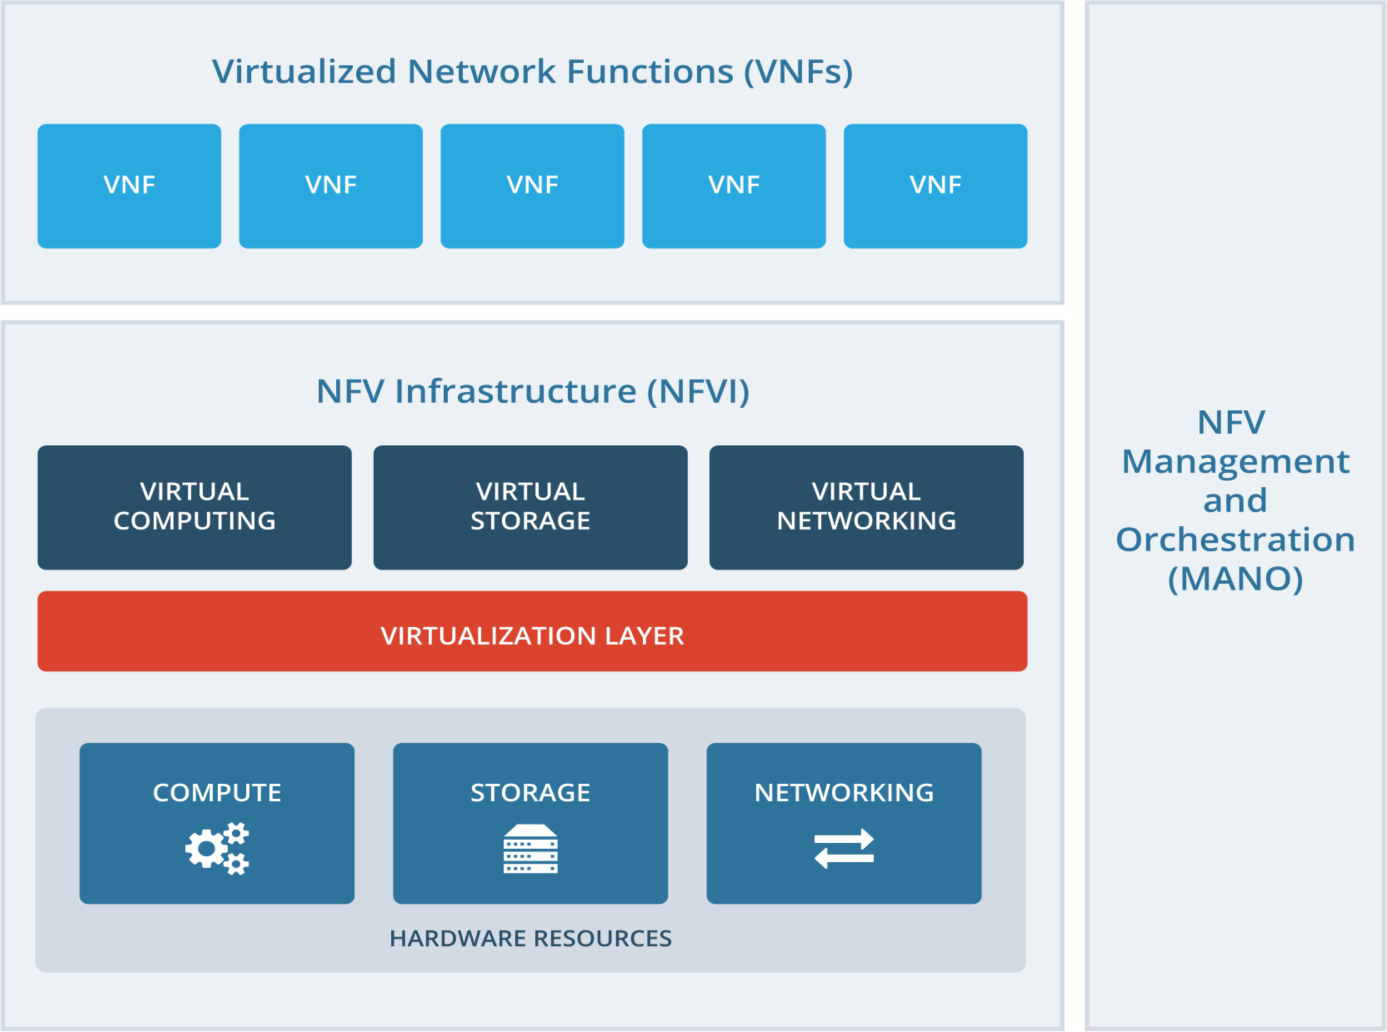
\includegraphics[width=1\linewidth]{OpenStackFoundationNFVReport}
		\caption{NFV functional overview\cite{openstack_nfv}}
		\label{fig:OpenStackFoundationNFVReport}
	\end{center}
	\vspace{-10pt}
\end{figure}

In an NFV environment, a virtual network function (VNF) takes on the responsibility of handling specific network functions that run on one or more virtual machines (VMs), on bare metal, or in containers, on top of the physical networking infrastructure.
A VNF can be an instance of any virtual hardware, for example: message router, CDN, DPI, Firewall, DNS...

The benefits of NFV stem from the fact that it runs on general purpose servers and switches in virtual machines or containers and is built with standard open APIs.

There are many ongoing NFV implementations. To keep it short, two of the NFV projects will be discussed.
\begin{itemize}
	\item Open Baton
	\item Tacker
\end{itemize}

\section{Open Baton - NFV Orchestrator}\label{sec:openbaton}
Open Baton is an European Telecommunications Standards Institute's (ETSI) NFV compliant Management and Orchestration (MANO) Framework.
It enables virtual Network Services deployments on top of the NFV infrastructure.

\begin{figure}[H]
	\begin{center}
		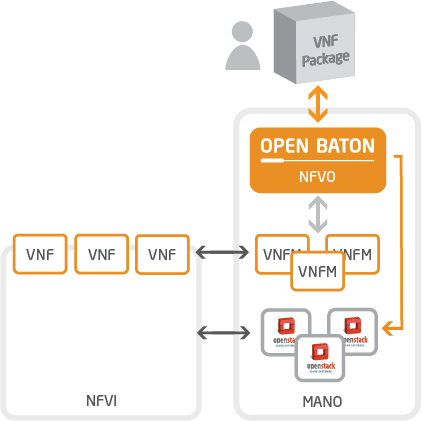
\includegraphics[width=1\linewidth]{openbaton_openstack}
		\caption{Placement of VNFM and VNF over the OpenStack Vitual Machines\cite{openBatonFeatures}}
		\label{fig:openbaton_openstack}
	\end{center}
	\vspace{-10pt}
\end{figure}

The Open Baton software is deployed over OpenStack with its own dashboard which would provide an easy to use web based VNF management console.
The VNF is configured on the virtual machine in the OpenStack IaaS.


\section{Tacker - OpenStack NFV Orchestration}\label{sec:tacker}

Tacker is an official OpenStack project building a Generic VNF Manager (VNFM) and a NFV Orchestrator (NFVO) to deploy and operate Network Services and Virtual Network Functions (VNFs) on an NFV infrastructure platform like OpenStack. It is based on ETSI MANO Architectural Framework and provides a functional stack to Orchestrate Network Services end-to-end using VNFs.


% !TEX root       = ./type_name.tex
% !TEX program    = pdflatex
% !TEX encoding   = utf-8
% !TEX spellcheck = de_DE_frami
%=======================================================================

\chapter{Conclusion}\label{ch:Conclusion}

OpenStack is an emerging and stable open source Cloud Infrastructure-as-a-Service operating solution.
OpenStack, with it's usage as Compute service- to create cloud based computing or Storage service- for cloud based storage solutions or both combined, is an easily deployable cloud operating solution with minimum infrastructure to start hosting the Cloud service.

As this thesis is focussed on scheduling algorithm of requested virtual instances, it can be observed from the logs in Appendix \ref{app:sec:filterschedulerlogtrace10vi} that, with the standard nova FilterScheduler, when a large number of virtual instance creation is requested, it iterates for that number of times to provide a placement decision one after the another. There is an opportunity for improvement to solve a large requests with minimum time and better mathematical modelling.

In the section \nameref{sec:comparision} of the chapter \nameref{ch:comparisionofbothscheduler}, it can be observed that the cPlex based scheduling algorithm is effective in providing a placement decision which would reduce the operating power expense of the OpenStack cloud cluster by minimising the active(powered on) number of hosts.

This is also effective in timely creation of large quantity of virtual instances compared to the existing standard nova scheduler.

This thesis is an approach to have a different possible solution in the scheduling algorithm which could be helpful to have constraint dependant scheduling.

This thesis can also be extended to have two different scheduling solutions depending on the number of requests for creation of the virtual instances.
With a condition based on quantity of instance creation, the selection of the scheduler driver can be switched at runtime.

If the "Live Migration" could work effectively, the scheduling algorithm could also include the migration of existing instances to re-arrange itself which would increase the available capacity on the hosts and place new instances with larger configuration requirements.
This could also be helpful for live migration of multiple virtual instances when the compute nodes needs a maintenance downtime.

The cloud computing is the growing field of interest which creates lots of opportunities for research and as well as the ideas for business.

%======================================================================
%:Literaturverzeichnis
%======================================================================
\newpage
\bibliographystyle{unsrtnat}
\bibliography{bib/literatur}


%======================================================================
%:Anhang (TODO)
%======================================================================
\appendix
\phantomsection{}
\addcontentsline{toc}{chapter}{\appendixname}
\addpart*{\appendixname}\label{p:anhang}

% !TEX root       = ./type_name.tex
% !TEX program    = pdflatex
% !TEX encoding   = utf-8
% !TEX spellcheck = de_DE_frami
%=======================================================================

\chapter{Router Configuration Content}\label{app:ch:Routerconfig}

In this Appendix \nameref{app:ch:Routerconfig}, the reader can find the specifically mentioned configuration for the router.

\section{Wireless configuration}\label{app:sec:wireless_config}
The Wireless configuration parameters set in the \verb|[OpenWrt]| are:
\begin{lstlisting}[frame=single]
config wifi-device 'radio0'
option type 'mac80211'
option channel '11'
option hwmode '11g'
option path 'platform/ar934x_wmac'
option htmode 'HT20'
option txpower '20'
option country 'DE'
option disabled '0'

config wifi-iface
option device 'radio0'
option mode 'ap'
option ssid 'OpenWrt'
option server '192.168.1.169'
option key 'testing123'
option encryption 'wpa2'
option network 'wifi'

config wifi-device 'radio1'
option type 'mac80211'
option channel '36'
option hwmode '11a'
option path 'pci0000:00/0000:00:00.0'
option htmode 'HT20'
option txpower '17'
option country 'DE'

config wifi-iface
option device 'radio1'
option mode 'ap'
option server '192.168.1.169'
option key 'testing123'
option ssid 'OpenWrt 5G'
option encryption 'wpa2'
option network 'wifi'
\end{lstlisting}
\section{Network configuration}\label{app:sec:Network_config}
The Network configuration parameters set in the \verb|[OpenWrt]| are:
\begin{lstlisting}[frame=single]
config interface 'loopback'
option ifname 'lo'
option proto 'static'
option ipaddr '127.0.0.1'
option netmask '255.0.0.0'

config globals 'globals'
option ula_prefix 'fd04:beb4:615d::/48'

config interface 'wan'
option ifname 'eth0.1'
option proto 'dhcp'

config interface 'wan6'
option ifname 'eth0.1'
option proto 'dhcpv6'

config interface 'lan'
option type 'bridge'
option ifname 'eth0.2'
option proto 'static'
option ipaddr '192.168.1.1'
option netmask '255.255.255.0'
option ip6assign '60'

config interface 'wifi'
option type 'bridge'
option ifname 'eth0.3'
option proto 'static'
option ipaddr '192.168.3.1'
option netmask '255.255.255.0'
option ip6assign '60'

config interface 'lan3'
option ifname 'eth0.3'

config interface 'lan4'
option ifname 'eth0.4'

config interface 'lan5'
option ifname 'eth0.5'

config switch
option name 'switch0'
option reset '1'
option enable_vlan '1'

config switch_vlan
option device 'switch0'
option vlan '1'
option ports '1 0t'
option vid '1'

config switch_vlan
option device 'switch0'
option vlan '2'
option ports '2 0t'
option ipaddr '192.168.3.1'
option netmask '255.255.255.0'
option ip6assign '60'

config interface 'lan3'
option ifname 'eth0.3'

config interface 'lan4'
option ifname 'eth0.4'

config interface 'lan5'
option ifname 'eth0.5'

config switch
option name 'switch0'
option reset '1'
option enable_vlan '1'

config switch_vlan
option device 'switch0'
option vlan '1'
option ports '1 0t'
option vid '1'

config switch_vlan
option device 'switch0'
option vlan '2'
option ports '2 0t'
option vid '2'

config switch_vlan
option device 'switch0'
option vlan '3'
option ports '3 0t'
option vid '3'

config switch_vlan
option device 'switch0'
option vlan '4'
option vid '4'
option ports '0t 4'

config switch_vlan
option device 'switch0'
option vlan '5'
option vid '5'
option ports '0t 5'
\end{lstlisting}
\section{DHCP configuration}\label{app:sec:DHCP_config}
The DHCP configuration parameters set in the \verb|[OpenWrt]| are:
\begin{lstlisting}[frame=single]

config dnsmasq
option domainneeded '1'
option boguspriv '1'
option filterwin2k '0'
option localise_queries '1'
option rebind_protection '1'
option rebind_localhost '1'
option local '/lan/'
option domain 'lan'
option expandhosts '1'
option nonegcache '0'
option authoritative '1'
option readethers '1'
option leasefile '/tmp/dhcp.leases'
option resolvfile '/tmp/resolv.conf.auto'
option localservice '1'

config dhcp 'lan'
option interface 'lan'
option start '100'
option limit '150'
option leasetime '12h'
option dhcpv6 'server'
option ra 'server'

config dhcp 'wifi'
option interface 'wifi'
option start '100'
option limit '150'
option leasetime '12h'
option dhcpv6 'server'
option ra 'server'

config dhcp 'wan'
option interface 'wan'
option ignore '1'

config odhcpd 'odhcpd'
option maindhcp '0'
option leasefile '/tmp/hosts/odhcpd'
option leasetrigger '/usr/sbin/odhcpd-update'

config dhcp 'lan4'
option interface 'lan4'
option ignore '1'


\end{lstlisting}

\chapter{RYU Verbose output}\label{app:ch:logs}

In this Appendix, the logs from the \verb|/tmp/log| file have been provided for different log purpose.

\section{RYU log trace}\label{app:sec:RYUlogtrace}

\begin{lstlisting}[frame=single, caption={The RYU Verbose log}, label={lst:RYUverboselog}]
loading app usr_seg.py
loading app ryu.controller.ofp_handler
instantiating app usr_seg.py of SimpleSwitch13
instantiating app ryu.controller.ofp_handler of OFPHandler
BRICK SimpleSwitch13
CONSUMES EventOFPPacketIn
CONSUMES EventOFPSwitchFeatures
BRICK ofp_event
PROVIDES EventOFPPacketIn TO {'SimpleSwitch13': set(['main'])}
PROVIDES EventOFPSwitchFeatures TO {'SimpleSwitch13': set(['config'])}
CONSUMES EventOFPEchoRequest
CONSUMES EventOFPPortStatus
CONSUMES EventOFPEchoReply
CONSUMES EventOFPSwitchFeatures
CONSUMES EventOFPPortDescStatsReply
CONSUMES EventOFPHello
CONSUMES EventOFPErrorMsg
connected socket:<eventlet.greenio.base.GreenSocket object at 0x7f42b40851d0> address:('192.168.1.1', 58461)
hello ev <ryu.controller.ofp_event.EventOFPHello object at 0x7f42b4085a90>
move onto config mode
EVENT ofp_event->SimpleSwitch13 EventOFPSwitchFeatures
switch features ev version=0x4,msg_type=0x6,msg_len=0x20,xid=0xf35c1db1,OFPSwitchFeatures(auxiliary_id=0,capabilities=79,datapath_id=176968783353910,n_buffers=256,n_tables=254)
move onto main mode
EVENT ofp_event->SimpleSwitch13 EventOFPPacketIn
packet truncated: only 170 of 342 bytes
Timestamp 2017-02-16 12:49:36.274578
Timestamp 2017-02-16 12:49:36.276005
outport_for_src tuple is None
Data is 00:26:9e:e2:b2:f8
packet in 176968783353910 00:26:9e:e2:b2:f8 ff:ff:ff:ff:ff:ff 2
DST is ff:ff:ff:ff:ff:ff
Out_Port before else flood condition None
Out_Port is Flooded 4294967291
Above actions Out_Port 4294967291
Actions is [OFPActionOutput(len=16,max_len=65509,port=4294967291,type=0)]
EVENT ofp_event->SimpleSwitch13 EventOFPPacketIn
EVENT ofp_event->SimpleSwitch13 EventOFPPacketIn
EVENT ofp_event->SimpleSwitch13 EventOFPPacketIn
EVENT ofp_event->SimpleSwitch13 EventOFPPacketIn
EVENT ofp_event->SimpleSwitch13 EventOFPPacketIn
EVENT ofp_event->SimpleSwitch13 EventOFPPacketIn
EVENT ofp_event->SimpleSwitch13 EventOFPPacketIn
EVENT ofp_event->SimpleSwitch13 EventOFPPacketIn
EVENT ofp_event->SimpleSwitch13 EventOFPPacketIn
Timestamp 2017-02-16 12:49:36.485248
Timestamp 2017-02-16 12:49:36.486536
outport_for_src tuple is None
Data is 00:26:9e:e2:b2:f8
packet in 176968783353910 00:26:9e:e2:b2:f8 ff:ff:ff:ff:ff:ff 2
DST is ff:ff:ff:ff:ff:ff
Out_Port before else flood condition None
Out_Port is Flooded 4294967291
Above actions Out_Port 4294967291
Actions is [OFPActionOutput(len=16,max_len=65509,port=4294967291,type=0)]
Timestamp 2017-02-16 12:49:36.490576
Timestamp 2017-02-16 12:49:36.491804
outport_for_src tuple is None
Data is 00:26:9e:e2:b2:f8
packet in 176968783353910 00:26:9e:e2:b2:f8 33:33:ff:a2:39:fe 2
DST is 33:33:ff:a2:39:fe
Out_Port before else flood condition None
Out_Port is Flooded 4294967291
Above actions Out_Port 4294967291
Actions is [OFPActionOutput(len=16,max_len=65509,port=4294967291,type=0)]
Timestamp 2017-02-16 12:49:36.495438
Timestamp 2017-02-16 12:49:36.496494
outport_for_src tuple is None
Data is 00:26:9e:e2:b2:f8
packet in 176968783353910 00:26:9e:e2:b2:f8 33:33:ff:00:07:5c 2
DST is 33:33:ff:00:07:5c
Out_Port before else flood condition None
Out_Port is Flooded 4294967291
Above actions Out_Port 4294967291
Actions is [OFPActionOutput(len=16,max_len=65509,port=4294967291,type=0)]
Timestamp 2017-02-16 12:49:36.499691
Timestamp 2017-02-16 12:49:36.500575
outport_for_src tuple is None
Data is a0:0b:ba:c9:9e:04
packet in 176968783353910 a0:0b:ba:c9:9e:04 ff:ff:ff:ff:ff:ff 1
DST is ff:ff:ff:ff:ff:ff
Out_Port before else flood condition None
Out_Port is Flooded 4294967291
Above actions Out_Port 4294967291
Actions is [OFPActionOutput(len=16,max_len=65509,port=4294967291,type=0)]
EVENT ofp_event->SimpleSwitch13 EventOFPPacketIn
packet truncated: only 170 of 350 bytes
Timestamp 2017-02-16 12:52:47.115680
Timestamp 2017-02-16 12:52:47.116894
outport_for_src tuple is ('2',)
Data is a0:0b:ba:c9:9e:04
packet in 176968783353910 a0:0b:ba:c9:9e:04 ff:ff:ff:ff:ff:ff 1
DST is ff:ff:ff:ff:ff:ff
Out_Port before else flood condition ('2',)
Setting Out_Port same as in table, changing flow 2
Above actions Out_Port 2
Actions is [OFPActionOutput(len=16,max_len=65509,port=2,type=0)]
Out_Port not flooded adding flow 
EVENT ofp_event->SimpleSwitch13 EventOFPPacketIn
Data is c8:5b:76:1b:ed:41
packet in 176968783353910 c8:5b:76:1b:ed:41 ff:ff:ff:ff:ff:ff 3
DST is ff:ff:ff:ff:ff:ff
Out_Port before else flood condition None
Out_Port is Flooded 4294967291
Above actions Out_Port 4294967291
Actions is [OFPActionOutput(len=16,max_len=65509,port=4294967291,type=0)]
Timestamp 2017-02-16 12:53:03.276915
Timestamp 2017-02-16 12:53:03.277904
outport_for_src tuple is None
Data is c8:5b:76:1b:ed:41
packet in 176968783353910 c8:5b:76:1b:ed:41 33:33:00:01:00:03 3
DST is 33:33:00:01:00:03
Out_Port before else flood condition None
Out_Port is Flooded 4294967291
Above actions Out_Port 4294967291
Actions is [OFPActionOutput(len=16,max_len=65509,port=4294967291,type=0)]
Timestamp 2017-02-16 12:53:03.282229
Timestamp 2017-02-16 12:53:03.283229
outport_for_src tuple is None
Data is c8:5b:76:1b:ed:41
packet in 176968783353910 c8:5b:76:1b:ed:41 01:00:5e:00:00:fb 3
DST is 01:00:5e:00:00:fb
Out_Port before else flood condition None
Out_Port is Flooded 4294967291
Above actions Out_Port 4294967291
Actions is [OFPActionOutput(len=16,max_len=65509,port=4294967291,type=0)]
EVENT ofp_event->SimpleSwitch13 EventOFPPacketIn
Timestamp 2017-02-16 12:54:32.618185
Timestamp 2017-02-16 12:54:32.619362
outport_for_src tuple is ('3',)
Data is c0:ee:fb:20:41:24
packet in 176968783353910 c0:ee:fb:20:41:24 01:00:5e:00:00:16 1
DST is 01:00:5e:00:00:16
Out_Port before else flood condition ('3',)
Setting Out_Port same as in table, changing flow 3
Above actions Out_Port 3
Actions is [OFPActionOutput(len=16,max_len=65509,port=3,type=0)]
Out_Port not flooded adding flow 
EVENT ofp_event->SimpleSwitch13 EventOFPPacketIn
Timestamp 2017-02-16 12:54:36.051777
Timestamp 2017-02-16 12:54:36.052886
outport_for_src tuple is ('3',)
Data is c0:ee:fb:20:41:24
packet in 176968783353910 c0:ee:fb:20:41:24 01:00:5e:00:00:fb 1
DST is 01:00:5e:00:00:fb
Out_Port before else flood condition ('3',)
Setting Out_Port same as in table, changing flow 3
Above actions Out_Port 3
Actions is [OFPActionOutput(len=16,max_len=65509,port=3,type=0)]
Out_Port not flooded adding flow 
EVENT ofp_event->SimpleSwitch13 EventOFPPacketIn
Timestamp 2017-02-16 12:55:09.360397
Timestamp 2017-02-16 12:55:09.361360
\end{lstlisting}


% !TEX root       = ./type_name.tex
% !TEX program    = pdflatex
% !TEX encoding   = utf-8
% !TEX spellcheck = de_DE_frami
%=======================================================================

\chapter{User Segregation Application code}\label{app:ch:app_code}

In this Appendix \nameref{app:ch:app_code}, the entire application code written in Python is listed here.


\begin{lstlisting}[language = Python, caption={The User Segregation Mac Learning Application}, label={lst:userseg-code}]
# Copyright (C) 2011 Nippon Telegraph and Telephone Corporation.
#
# Licensed under the Apache License, Version 2.0 (the "License");
# you may not use this file except in compliance with the License.
# You may obtain a copy of the License at
#
#    http://www.apache.org/licenses/LICENSE-2.0
#
# Unless required by applicable law or agreed to in writing, software
# distributed under the License is distributed on an "AS IS" BASIS,
# WITHOUT WARRANTIES OR CONDITIONS OF ANY KIND, either express or
# implied.
# See the License for the specific language governing permissions and
# limitations under the License.
import MySQLdb
import sys
import datetime
from ryu.base import app_manager
from ryu.controller import ofp_event
from ryu.controller.handler import CONFIG_DISPATCHER, MAIN_DISPATCHER
from ryu.controller.handler import set_ev_cls
from ryu.ofproto import ofproto_v1_3
from ryu.lib.packet import packet
from ryu.lib.packet import ethernet
from ryu.lib.packet import ether_types
from ryu.lib.packet import udp



class SimpleSwitch13(app_manager.RyuApp):
	OFP_VERSIONS = [ofproto_v1_3.OFP_VERSION]

	def __init__(self, *args, **kwargs):
		super(SimpleSwitch13, self).__init__(*args, **kwargs)
		self.mac_to_port = {}

	@set_ev_cls(ofp_event.EventOFPSwitchFeatures, CONFIG_DISPATCHER)
	def switch_features_handler(self, ev):
		datapath = ev.msg.datapath
		ofproto = datapath.ofproto
		parser = datapath.ofproto_parser

		# install table-miss flow entry
		#
		# We specify NO BUFFER to max_len of the output action due to
		# OVS bug. At this moment, if we specify a lesser number, e.g.,
		# 128, OVS will send Packet-In with invalid buffer_id and
		# truncated packet data. In that case, we cannot output packets
		# correctly.  The bug has been fixed in OVS v2.1.0.
		match = parser.OFPMatch()
		actions = [parser.OFPActionOutput(ofproto.OFPP_CONTROLLER, ofproto.OFPCML_NO_BUFFER)]
		self.add_flow(datapath, 0, match, actions)

	def add_flow(self, datapath, priority, match, actions, buffer_id=None):
		ofproto = datapath.ofproto
		parser = datapath.ofproto_parser

		inst = [parser.OFPInstructionActions(ofproto.OFPIT_APPLY_ACTIONS, actions)]
		if buffer_id: 
			mod = parser.OFPFlowMod(datapath=datapath, buffer_id=buffer_i , priority=priority, match=match, instructions=inst)
		else:
			mod = parser.OFPFlowMod(datapath=datapath, priority=priority, match=match, instructions=inst)
			
		datapath.send_msg(mod)

	@set_ev_cls(ofp_event.EventOFPPacketIn, MAIN_DISPATCHER)
	def _packet_in_handler(self, ev):
	# If you hit this you might want to increase
	# the "miss_send_length" of your switch

		if ev.msg.msg_len < ev.msg.total_len:
			self.logger.debug("packet truncated: only %s of %s bytes", ev.msg.msg_len, ev.msg.total_len)
		msg = ev.msg
		datapath = msg.datapath
		ofproto = datapath.ofproto
		parser = datapath.ofproto_parser
		in_port = msg.match['in_port']

		pkt = packet.Packet(msg.data)
		eth = pkt.get_protocols(ethernet.ethernet)[0]
		udp_payload = pkt.get_protocols(udp.udp)


		if eth.ethertype == ether_types.ETH_TYPE_LLDP:
			# ignore lldp packet
			return
		dst = eth.dst
		src = eth.src

		dpid = datapath.id
		self.mac_to_port.setdefault(dpid, {})
	

	#creating a mysql connection to database -last edit 17/11

	connection = MySQLdb.connect(host = "192.168.1.169", user = "freerad", passwd = "pass", db = "radius")
	cursor = connection.cursor ()
	cursor.execute ("SELECT portid FROM radcheck WHERE username IN (SELECT user FROM radpostauth WHERE CallingStationId = %s AND id = (SELECT MAX(id) from radpostauth) )", src)
	outport_for_src = cursor.fetchone ()

	cursor.close()
	connection.close ()
	# Mysql verification end


		# learn a mac address to avoid FLOOD next time.
		self.mac_to_port[dpid][src] = in_port
	
	if dst in self.mac_to_port[dpid]:
		test = self.mac_to_port[dpid][dst]
		
		if outport_for_src != None and all(outport_for_src):
			if int(outport_for_src[0]) == self.mac_to_port[dpid][dst]:
				out_port = self.mac_to_port[dpid][dst]

			else:

				return

		else:
		#except (TypeError,UnboundLocalError):		
			out_port = self.mac_to_port[dpid][dst]		

	else:

		if outport_for_src != None and all(outport_for_src): out_port = int(outport_for_src[0])

		else:
		#except (TypeError,UnboundLocalError):

			out_port = ofproto.OFPP_FLOOD

		actions = [parser.OFPActionOutput(out_port)]


		# install a flow to avoid packet_in next time
		if out_port != ofproto.OFPP_FLOOD:

			match = parser.OFPMatch(in_port=in_port, eth_dst=dst)
			#match = parser.OFPMatch(in_port=in_port, eth_dst='a0:f3:c1:77:d8:36')
			# verify if we have a valid buffer_id, if yes avoid to send both
			# flow_mod & packet_out
			if msg.buffer_id != ofproto.OFP_NO_BUFFER:
				self.add_flow(datapath, 1, match, actions, msg.buffer_id)
				return
			else:
				self.add_flow(datapath, 1, match, actions)
		data = None

		if msg.buffer_id == ofproto.OFP_NO_BUFFER:
			data = msg.data

		out = parser.OFPPacketOut(datapath=datapath, buffer_id=msg.buffer_id, in_port=in_port, actions=actions, data=data)
		datapath.send_msg(out)

\end{lstlisting}






%======================================================================
%:Selbstständigkeitserklärung
%======================================================================
\addchap{Versicherung}

Hiermit versichere ich, dass ich die vorliegende Arbeit ohne unzulässige Hilfe Dritter und ohne
Benutzung anderer als der angegebenen Hilfsmittel angefertigt habe; die aus fremden Quellen direkt
oder indirekt übernommenen Gedanken sind als solche kenntlich gemacht.\\
Bei der Auswahl und Auswertung des Materials sowie bei der Herstellung des Manuskripts habe ich
Unterstützungsleistungen von folgenden Personen erhalten: \\[2ex]
\hspace*{\fill}keine\hspace*{\fill}\\[2ex]
Weitere Personen waren an der Abfassung der vorliegenden Arbeit nicht beteiligt. Die Hilfe eines
Promotionsberaters habe ich nicht in Anspruch genommen. Weitere Personen haben von mir keine
geldwerten Leistungen für Arbeiten erhalten, die im Zusammenhang mit dem Inhalt der vorgelegten
Dissertation stehen.

Die Arbeit wurde bisher weder im Inland noch im Ausland in gleicher oder ähnlicher Form einer
anderen Prüfungsbehörde vorgelegt.

\vspace{4ex}
\begin{flushleft}
\dcplace, \dcdate\\[8ex]
\newlength\us\settowidth{\us}{-\dcauthorfirstname~\dcauthorlastname-}
\begin{tabular}{p{\us}}\midrule
\centering\footnotesize \dcauthorfirstname~\dcauthorlastname{}
\end{tabular}
\end{flushleft}

\end{document}
%=======================================================================
% vim: ts=2:sw=2:sts=2:expandtab:wrapmargin=2:tw=120

